\clearpage
\pagenumbering{arabic}
\setcounter{page}{1}

\rhead{Vedlegg B side \thepage}

\section{Azure Data Science Virtual Machine med Ubuntu Linux 18.04}
\label{appendix:azure}

Følgende steg under beskriver hvordan man lager en Data Science Virtual Machine instanse med Ubuntu Linux 18.04. Denne informasjonen er fra 	kurset Deep Learning with PyTorch. \cite{Mallick m.fl. 2020}

Before proceeding, it is worth noting that the instance should be shut down when you are not using them. Since the GPU instances are expensive, it may use up your credits very fast. So, remember to shut down the instance after using it.

1. Login to the Azure portal using \url{portal.azure.com}. You should see a dashboard similar to this:

\begin{figure}[H]
\begin{center} 
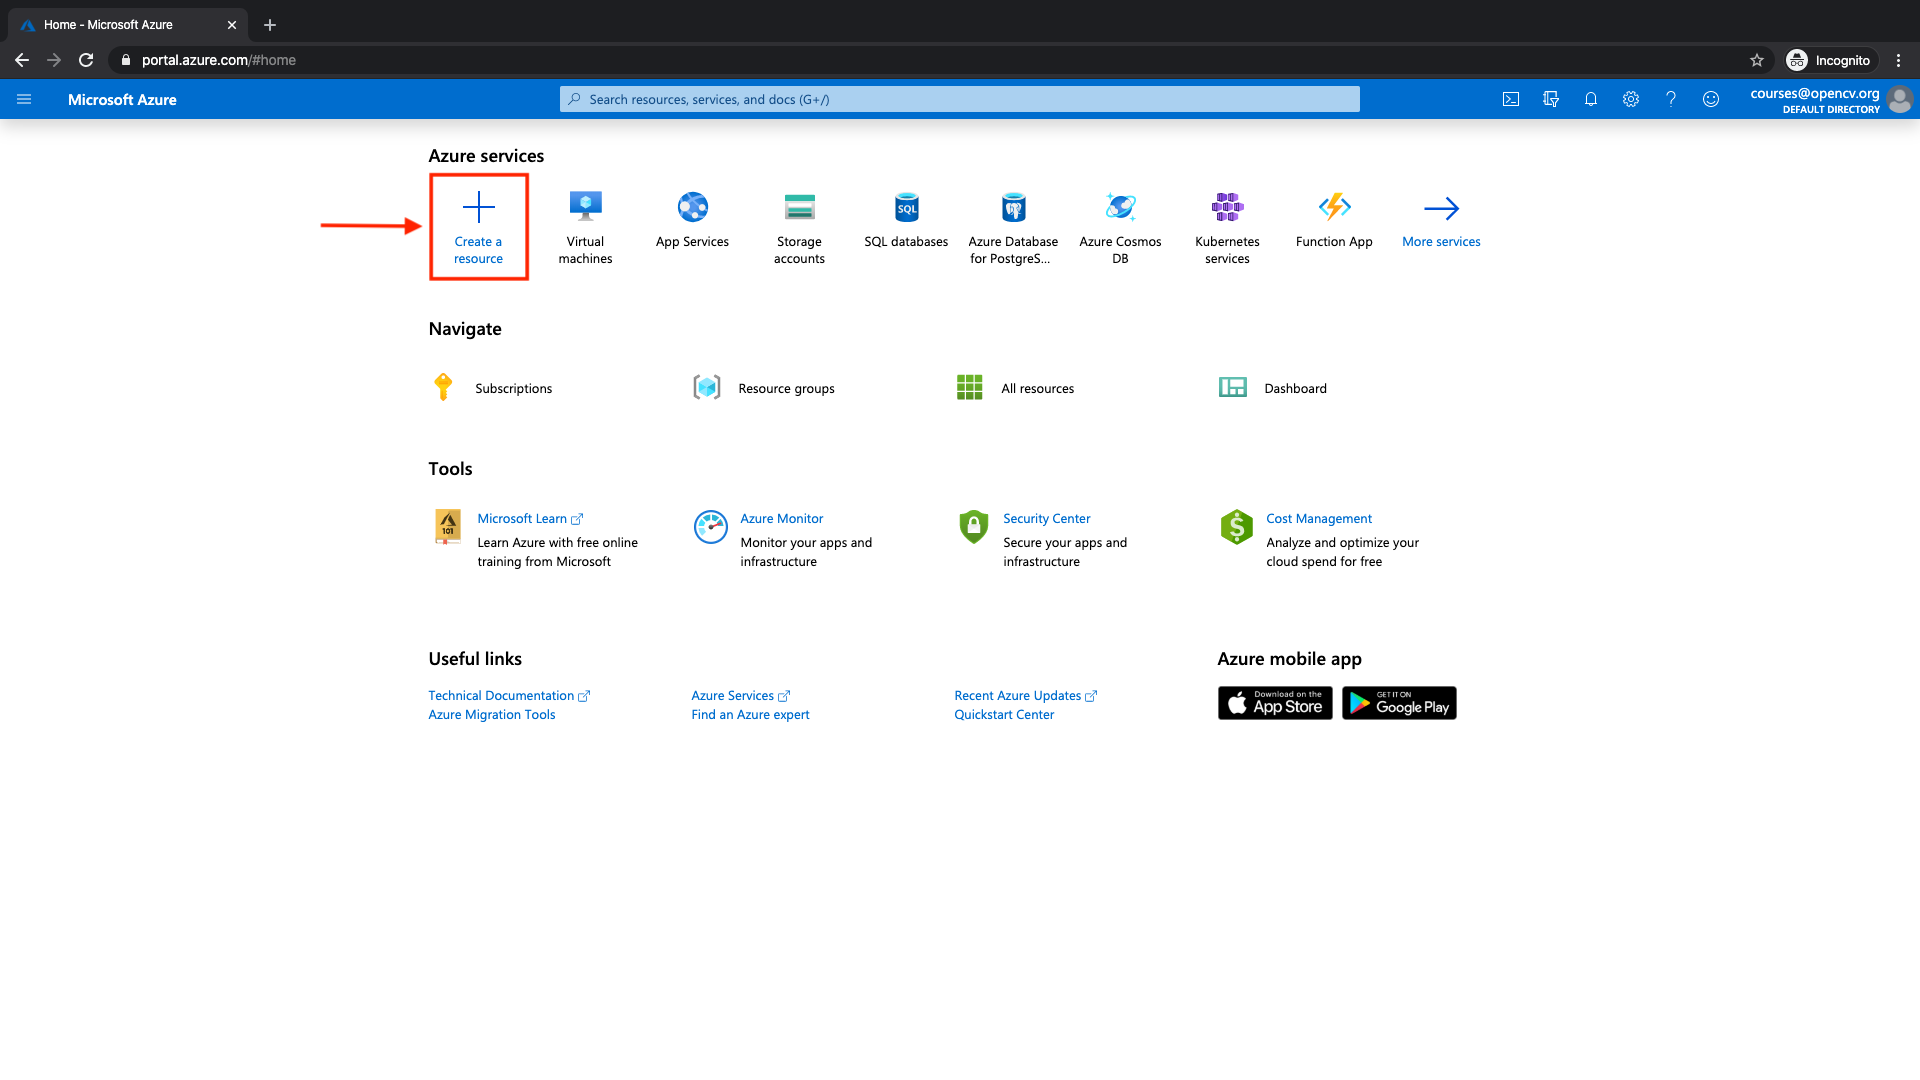
\includegraphics[scale=0.20]{figures/vm1}
%\caption{\small \sl . \cite{Mallick m.fl. 2020} \label{fig:azure}}
\end{center}
\end{figure}

2. Search for Data Science Virtual Machine and choose the one with 18.04 as shown.

\begin{figure}[H]
\begin{center} 
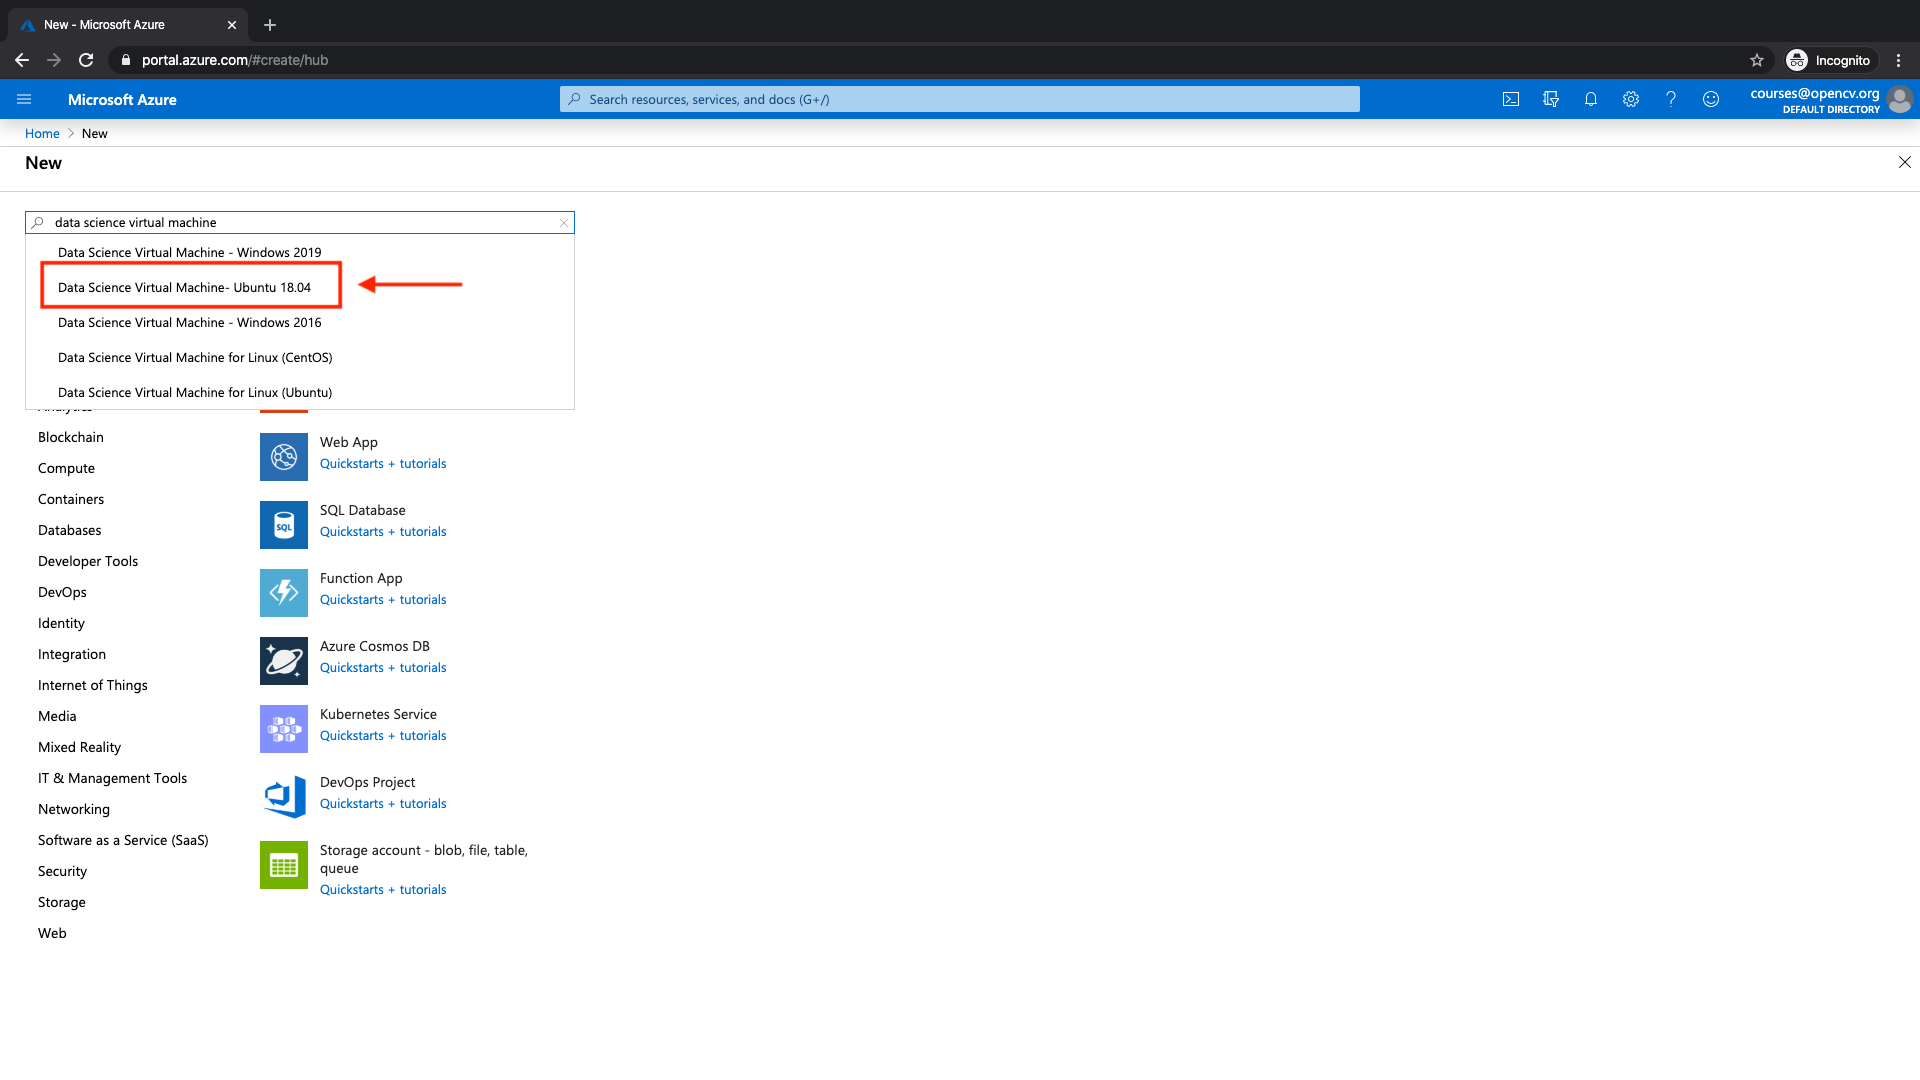
\includegraphics[scale=0.20]{figures/vm2}
%\caption{\small \sl . \cite{Mallick m.fl. 2020} \label{fig:azure}}
\end{center}
\end{figure}

3. Once you select the VM image, you can click on Create.

\begin{figure}[H]
\begin{center} 
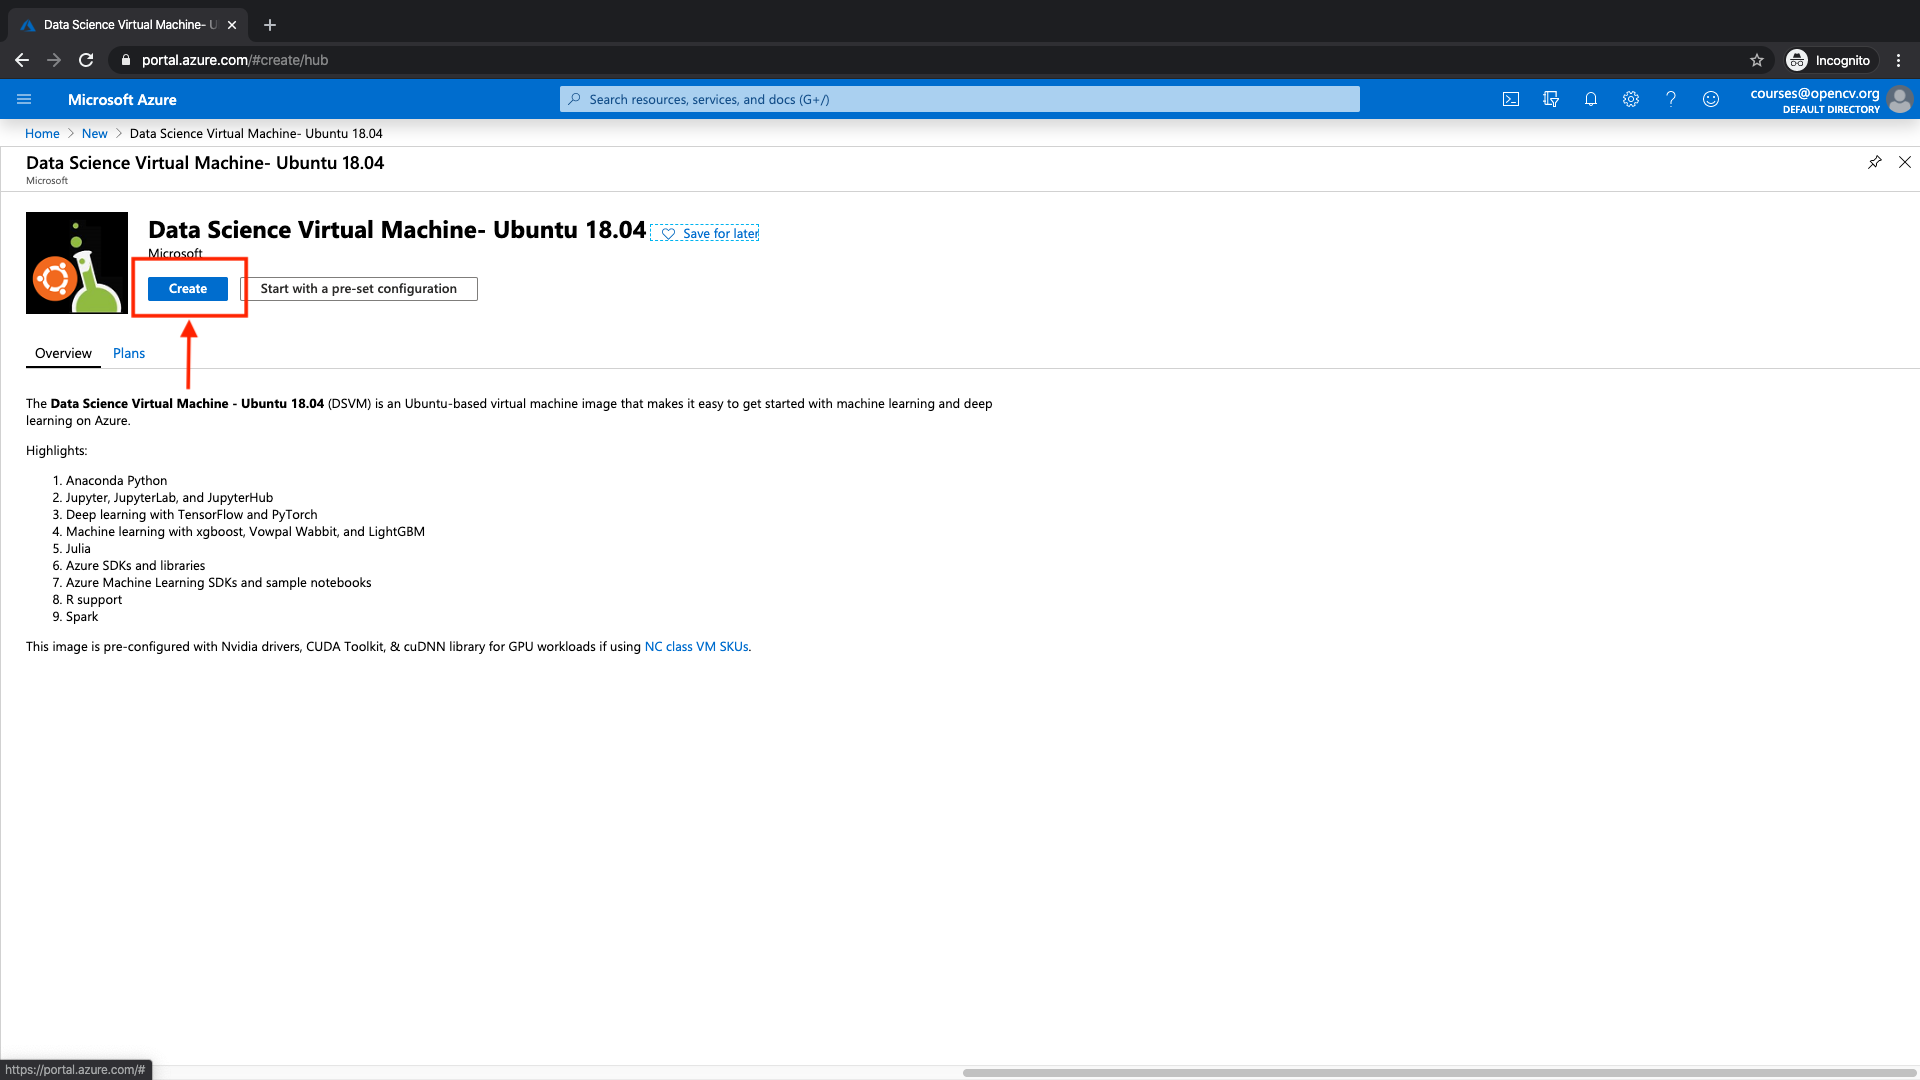
\includegraphics[scale=0.20]{figures/vm3}
%\caption{\small \sl . \cite{Mallick m.fl. 2020} \label{fig:azure}}
\end{center}
\end{figure}

4. Create New Resource Group as shown

\begin{figure}[H]
\begin{center} 
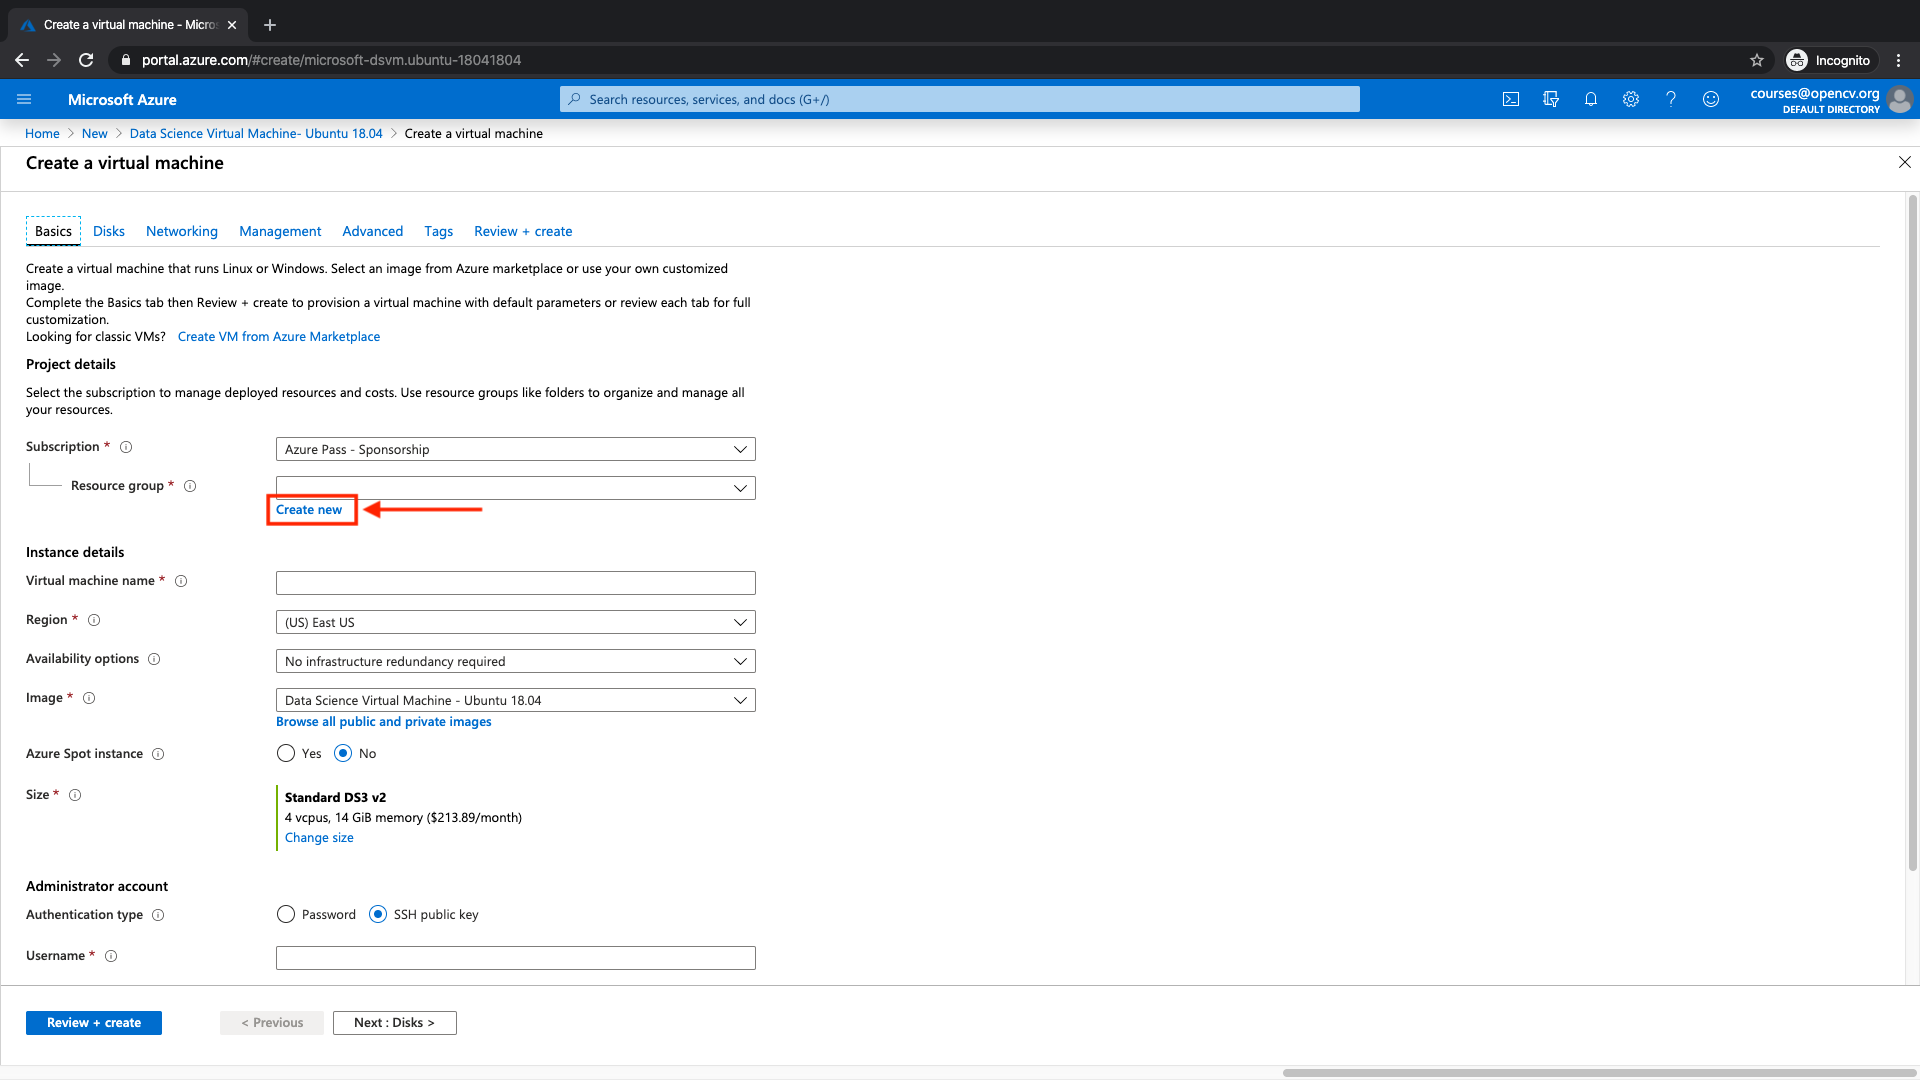
\includegraphics[scale=0.20]{figures/vm4}
%\caption{\small \sl . \cite{Mallick m.fl. 2020} \label{fig:azure}}
\end{center}
\end{figure}

5. You can provide any name of your choice. This can be reused when you create more VMs later.

\begin{figure}[H]
\begin{center} 
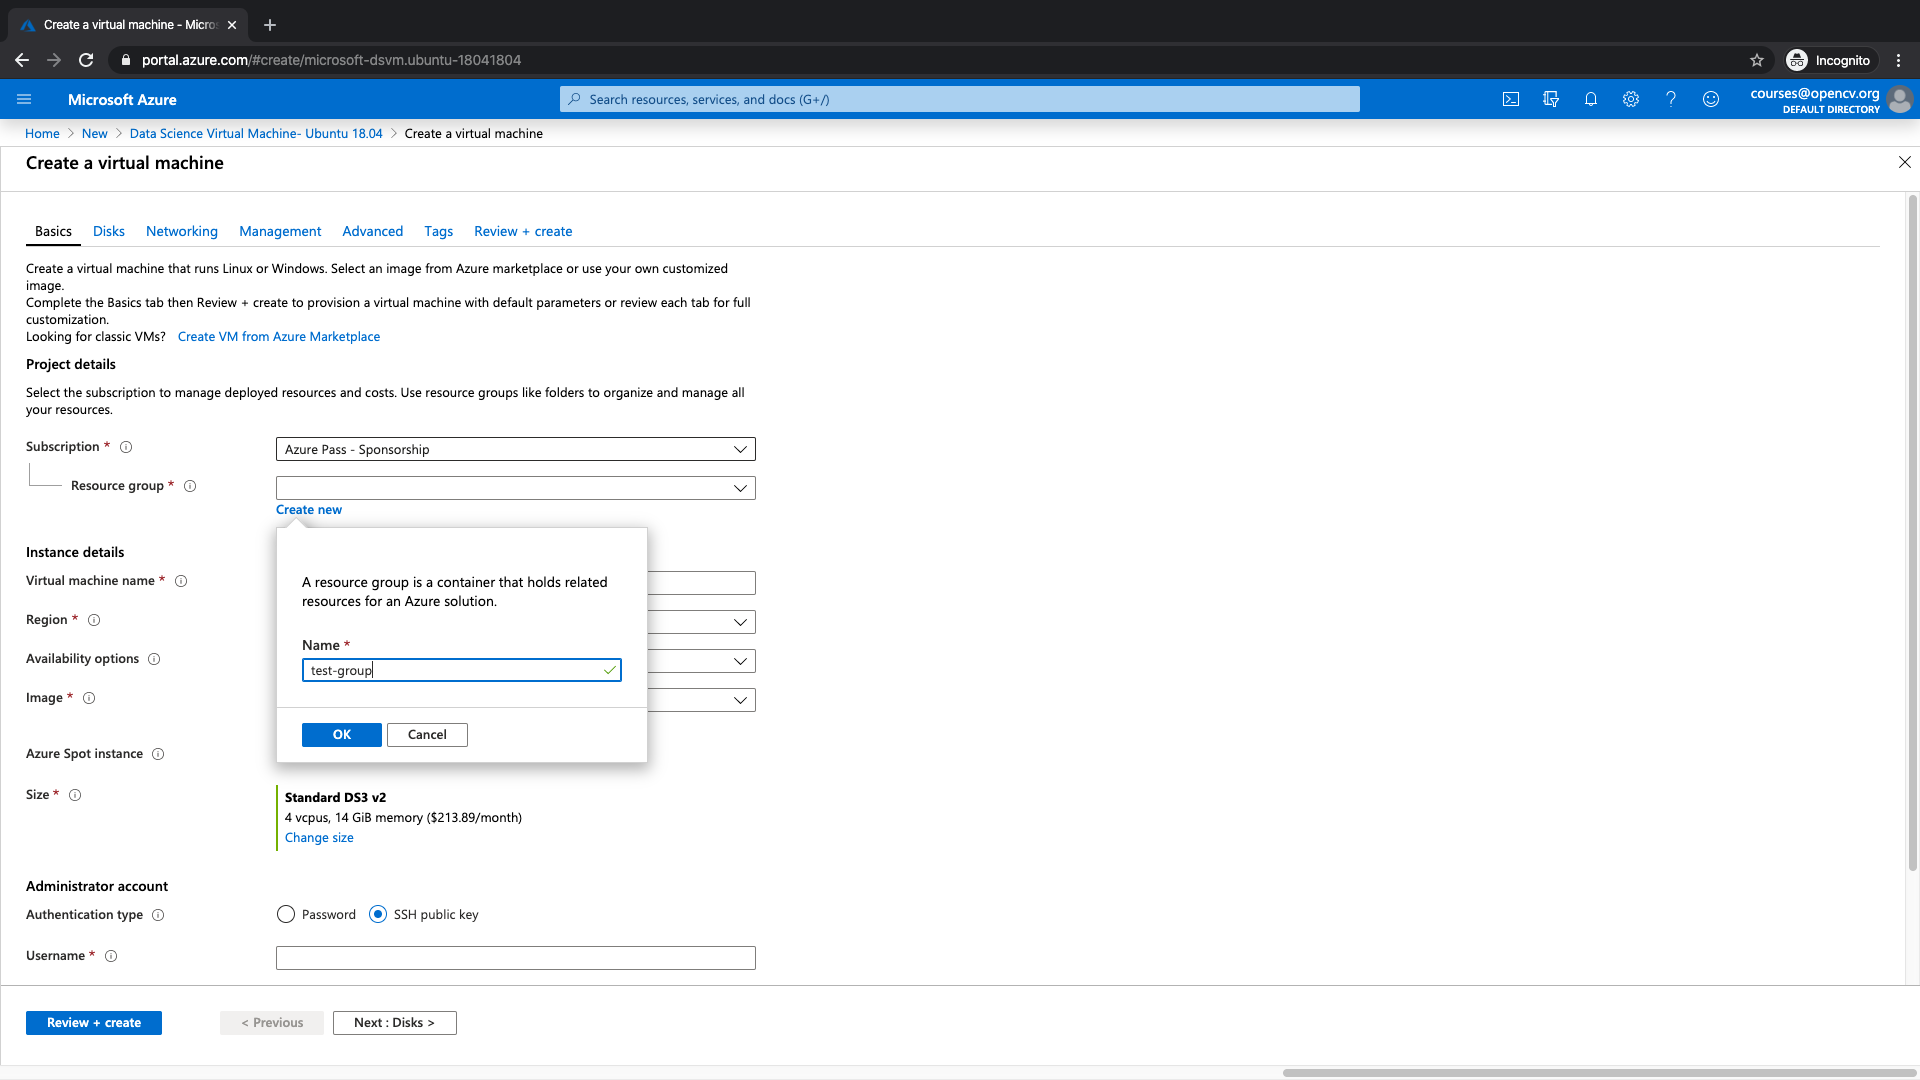
\includegraphics[scale=0.20]{figures/vm5}
%\caption{\small \sl . \cite{Mallick m.fl. 2020} \label{fig:azure}}
\end{center}
\end{figure}

6. Provide a name for your machine

\begin{figure}[H]
\begin{center} 
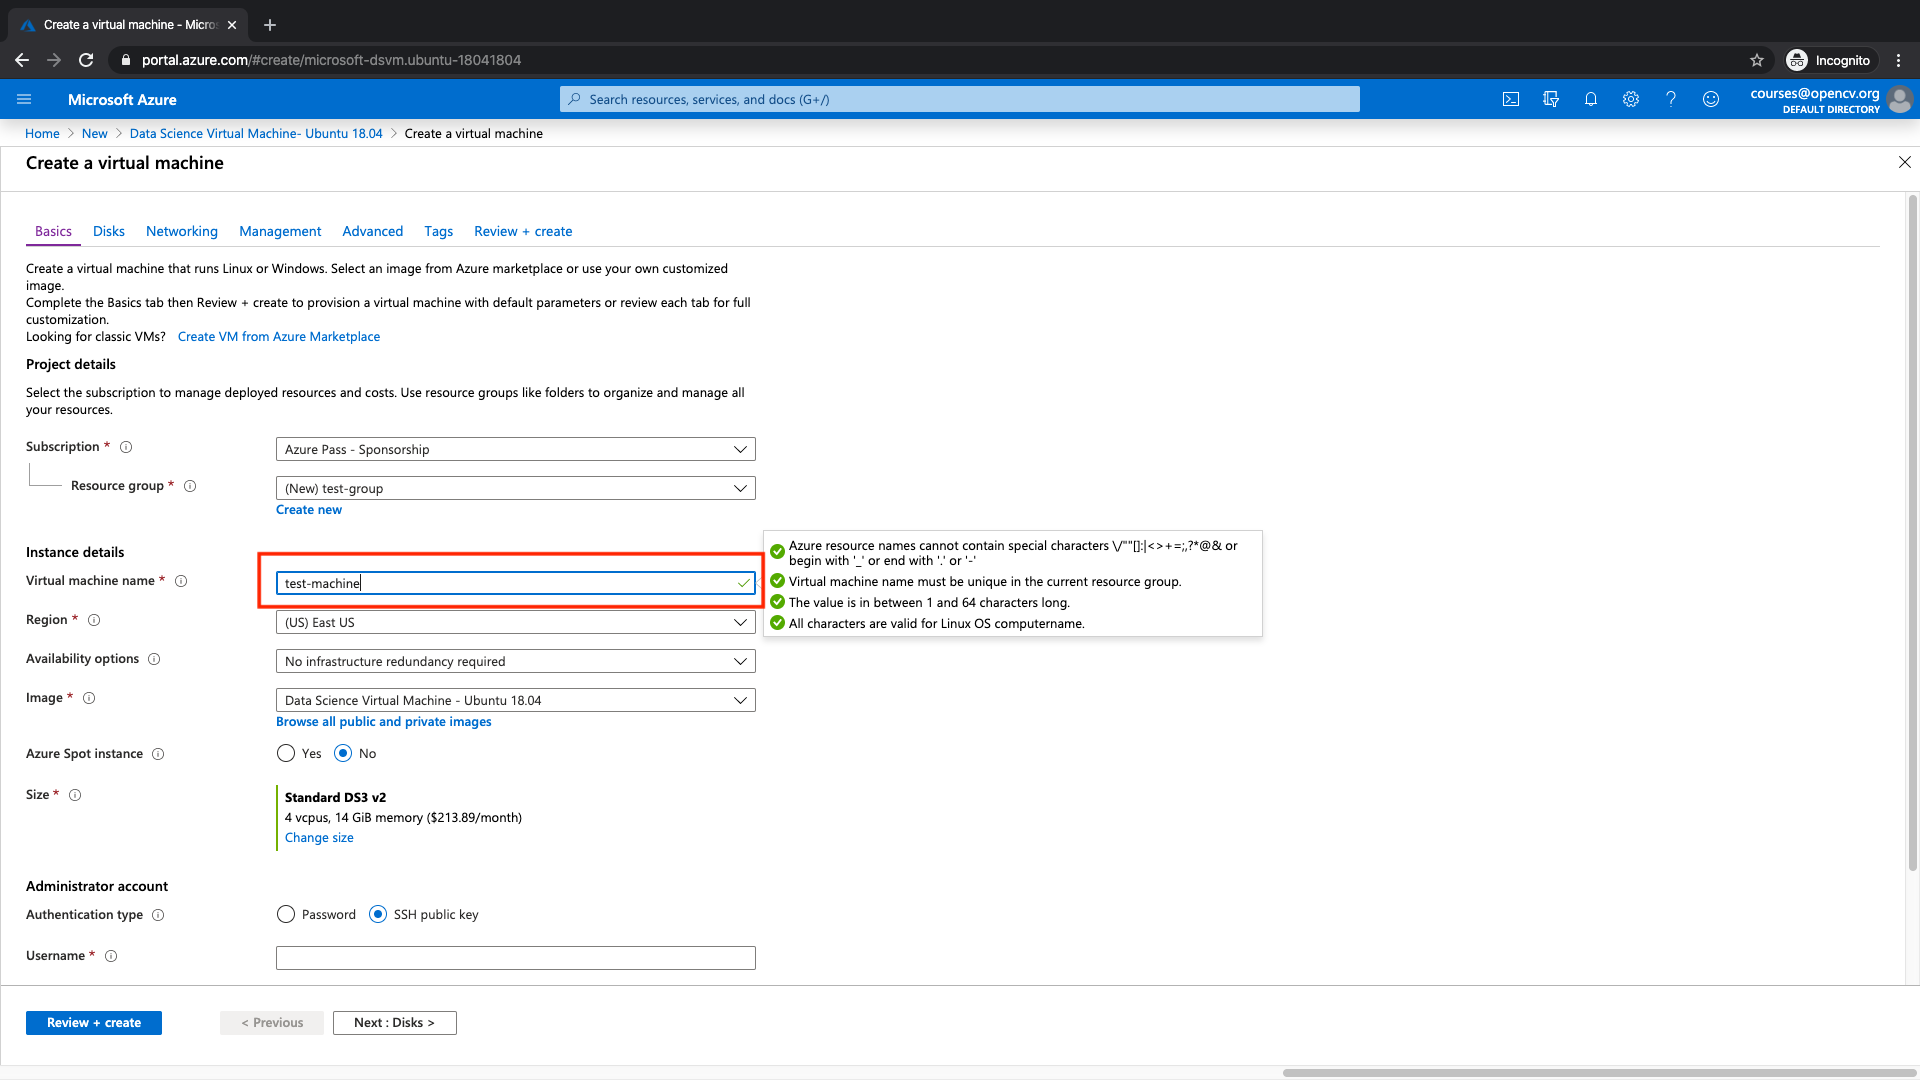
\includegraphics[scale=0.20]{figures/vm6}
%\caption{\small \sl . \cite{Mallick m.fl. 2020} \label{fig:azure}}
\end{center}
\end{figure}

7. Select the Region.
A few important points to note about regions:

1. All types of instances are not available in all regions. Generally, regions in the US and Europe have instances of all types. So, it is advisable to select US/Europe regions even if you are not from these regions.

2. An example where you may want to switch regions is that you may not find the required instance in that particular region at any given time. For example, I was able to select NC6\_Promo instance from US East. But when I checked later, there were no available instances of type NC6\_Promo in US East, so I had to choose US West 2.

3. Pricing varies among different regions. I have generally found US East, US West 2, and US North Central to be cheaper.

Here, we have selected US East region.

\begin{figure}[H]
\begin{center} 
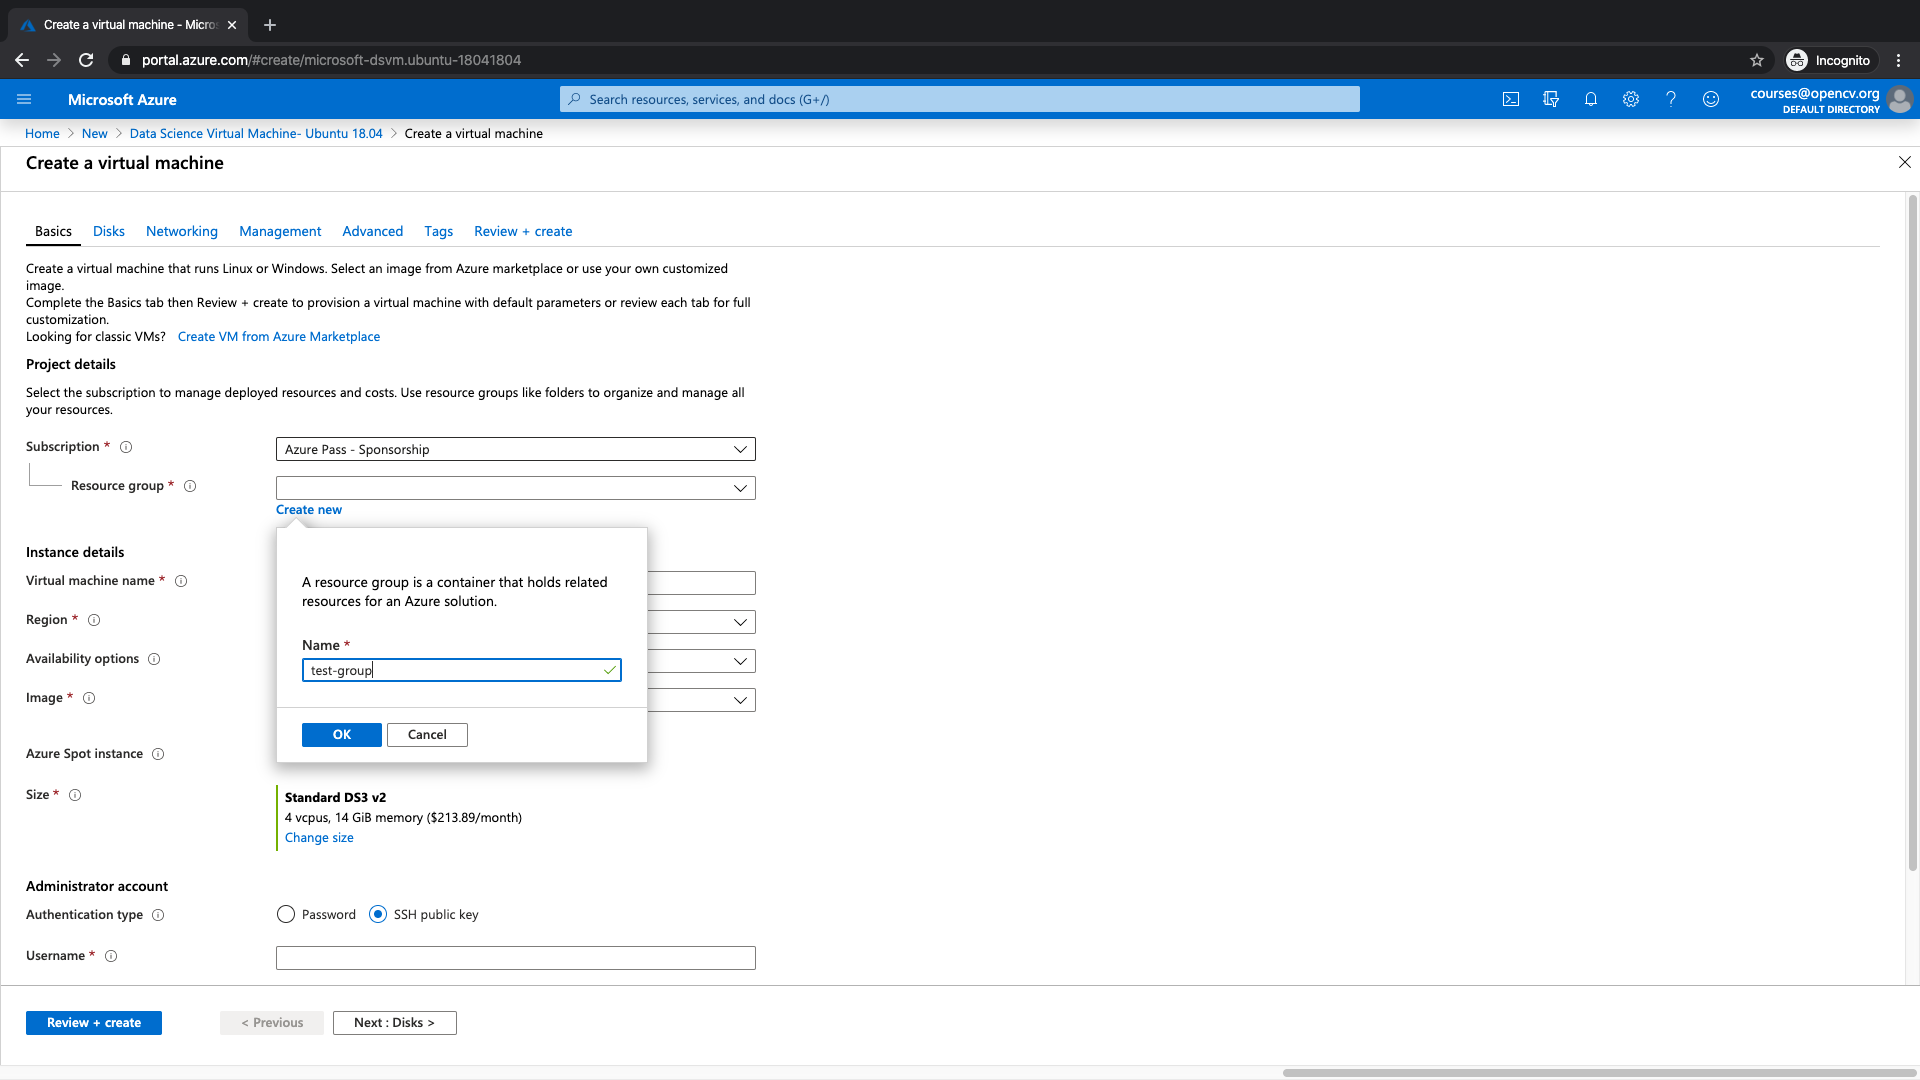
\includegraphics[scale=0.20]{figures/vm5}
%\caption{\small \sl . \cite{Mallick m.fl. 2020} \label{fig:azure}}
\end{center}
\end{figure}

8. Change the type of Instance
We want to use a GPU instance. Low-cost GPU instances are named NCx\_Promo where x can be 6, 12 etc. We will select NC6\_Promo. 

\begin{figure}[H]
\begin{center} 
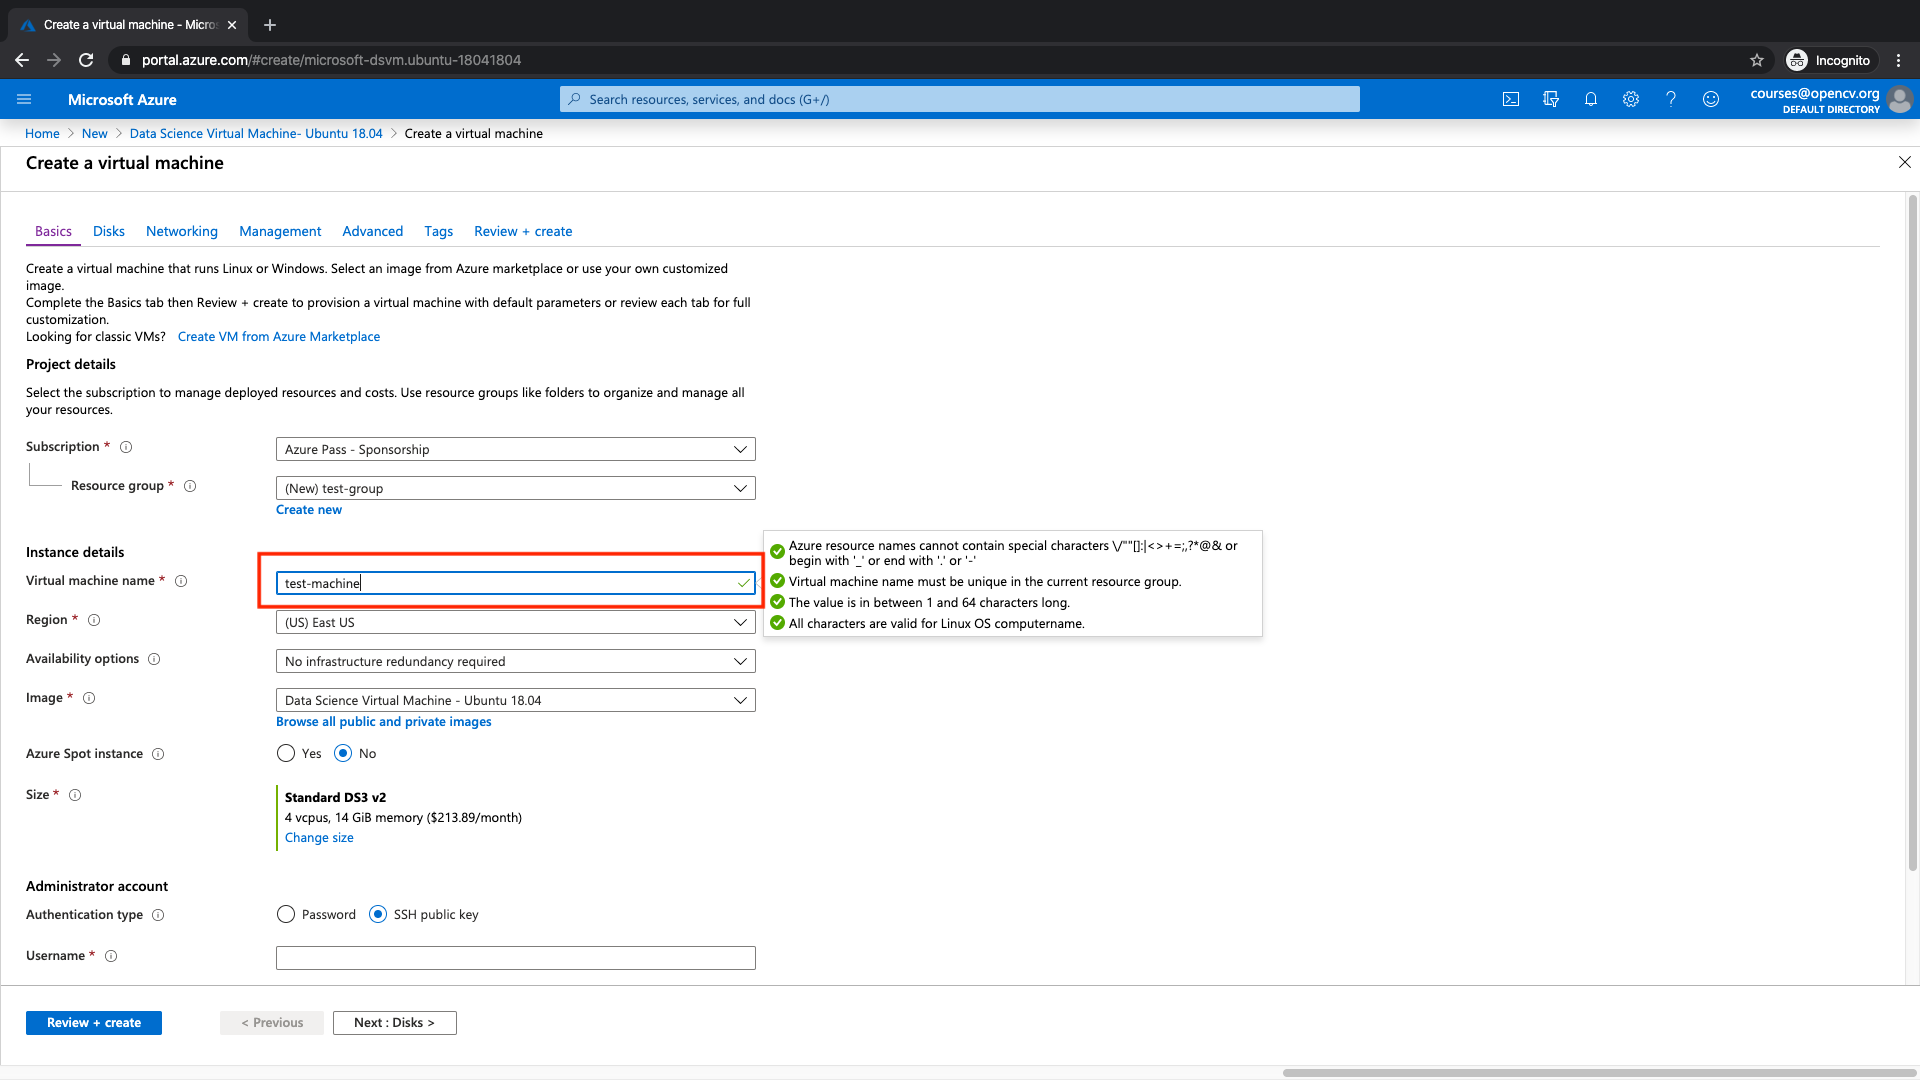
\includegraphics[scale=0.20]{figures/vm6}
%\caption{\small \sl . \cite{Mallick m.fl. 2020} \label{fig:azure}}
\end{center}
\end{figure}

Note that if you do not find NC6\_Promo in the selected region then you should try changing the region until you find the desired instance type.

Let us change the instance type.

9. Clear default filters

\begin{figure}[H]
\begin{center} 
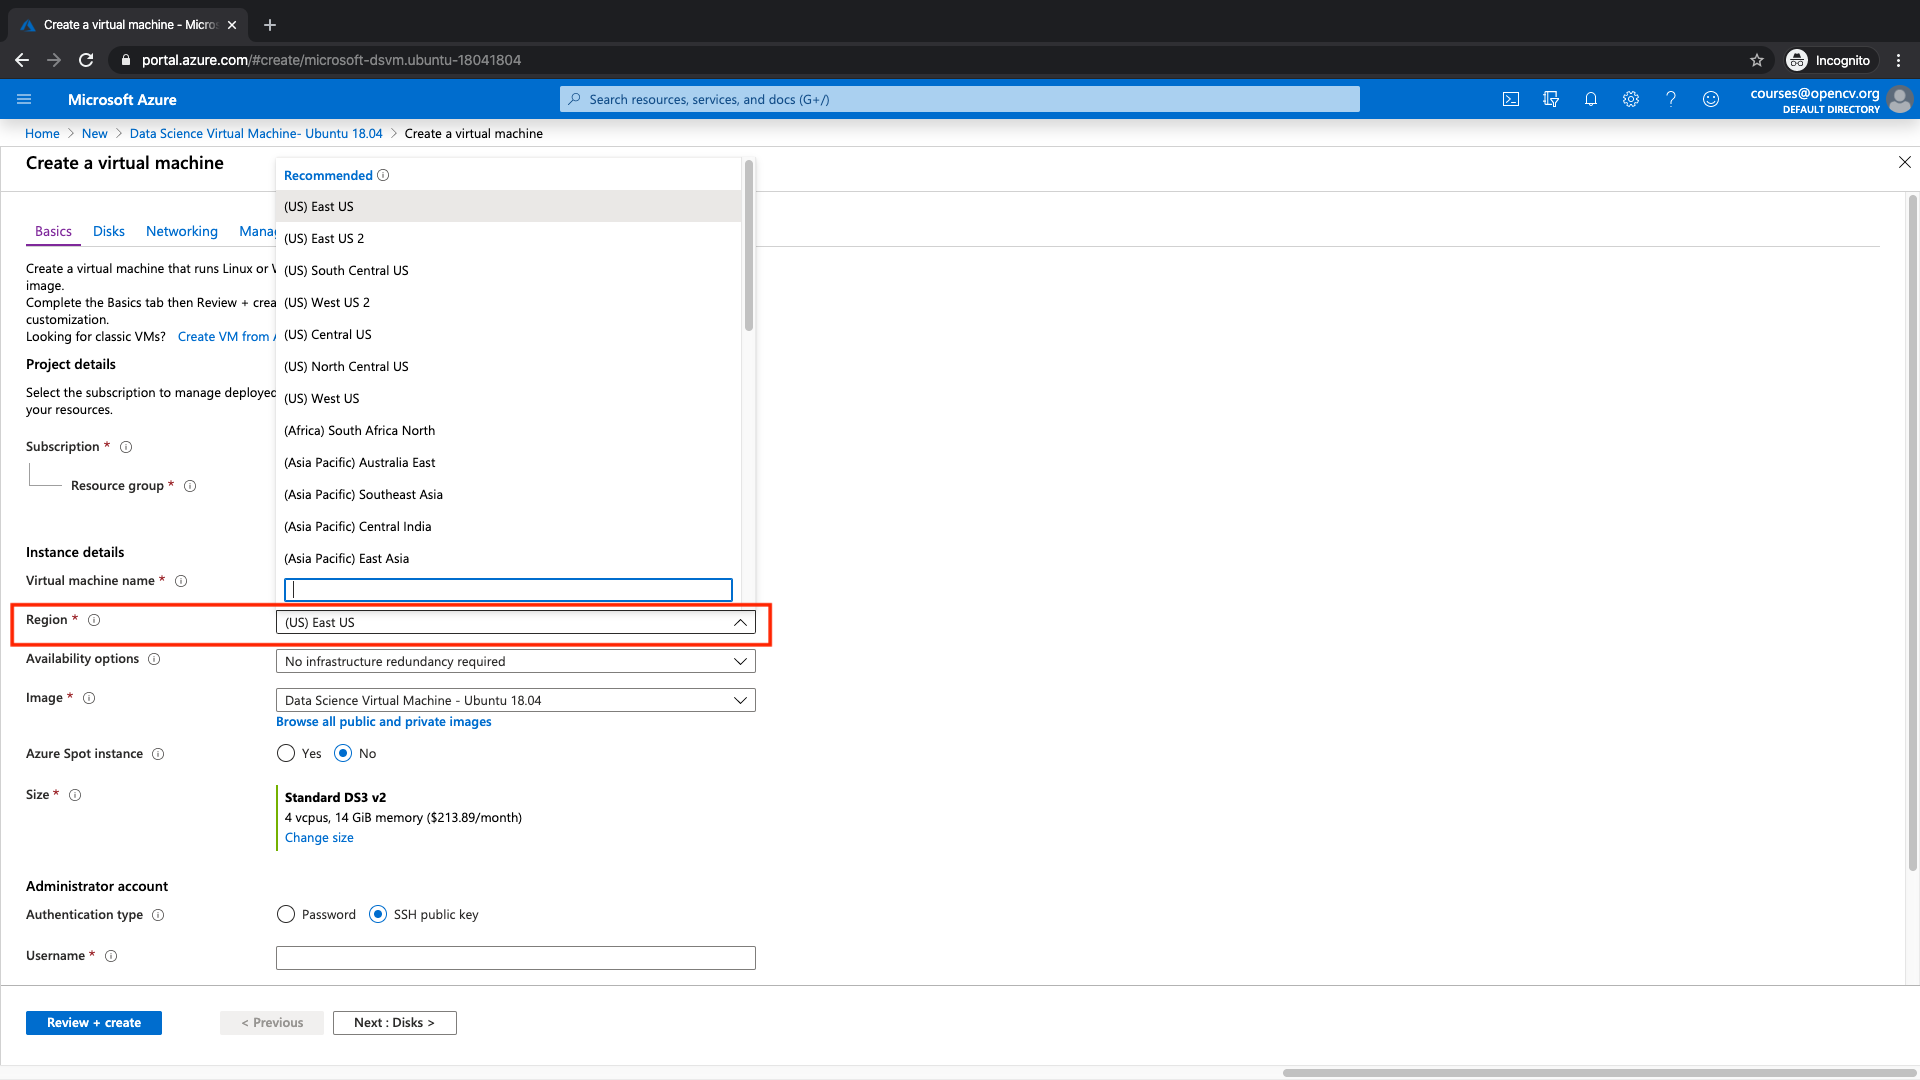
\includegraphics[scale=0.20]{figures/vm7}
%\caption{\small \sl . \cite{Mallick m.fl. 2020} \label{fig:azure}}
\end{center}
\end{figure}

10. Add Filter for GPU instances
We will apply the filter of GPU family of instances as shown in the 3 screenshots below.

\begin{figure}[H]
\begin{center} 
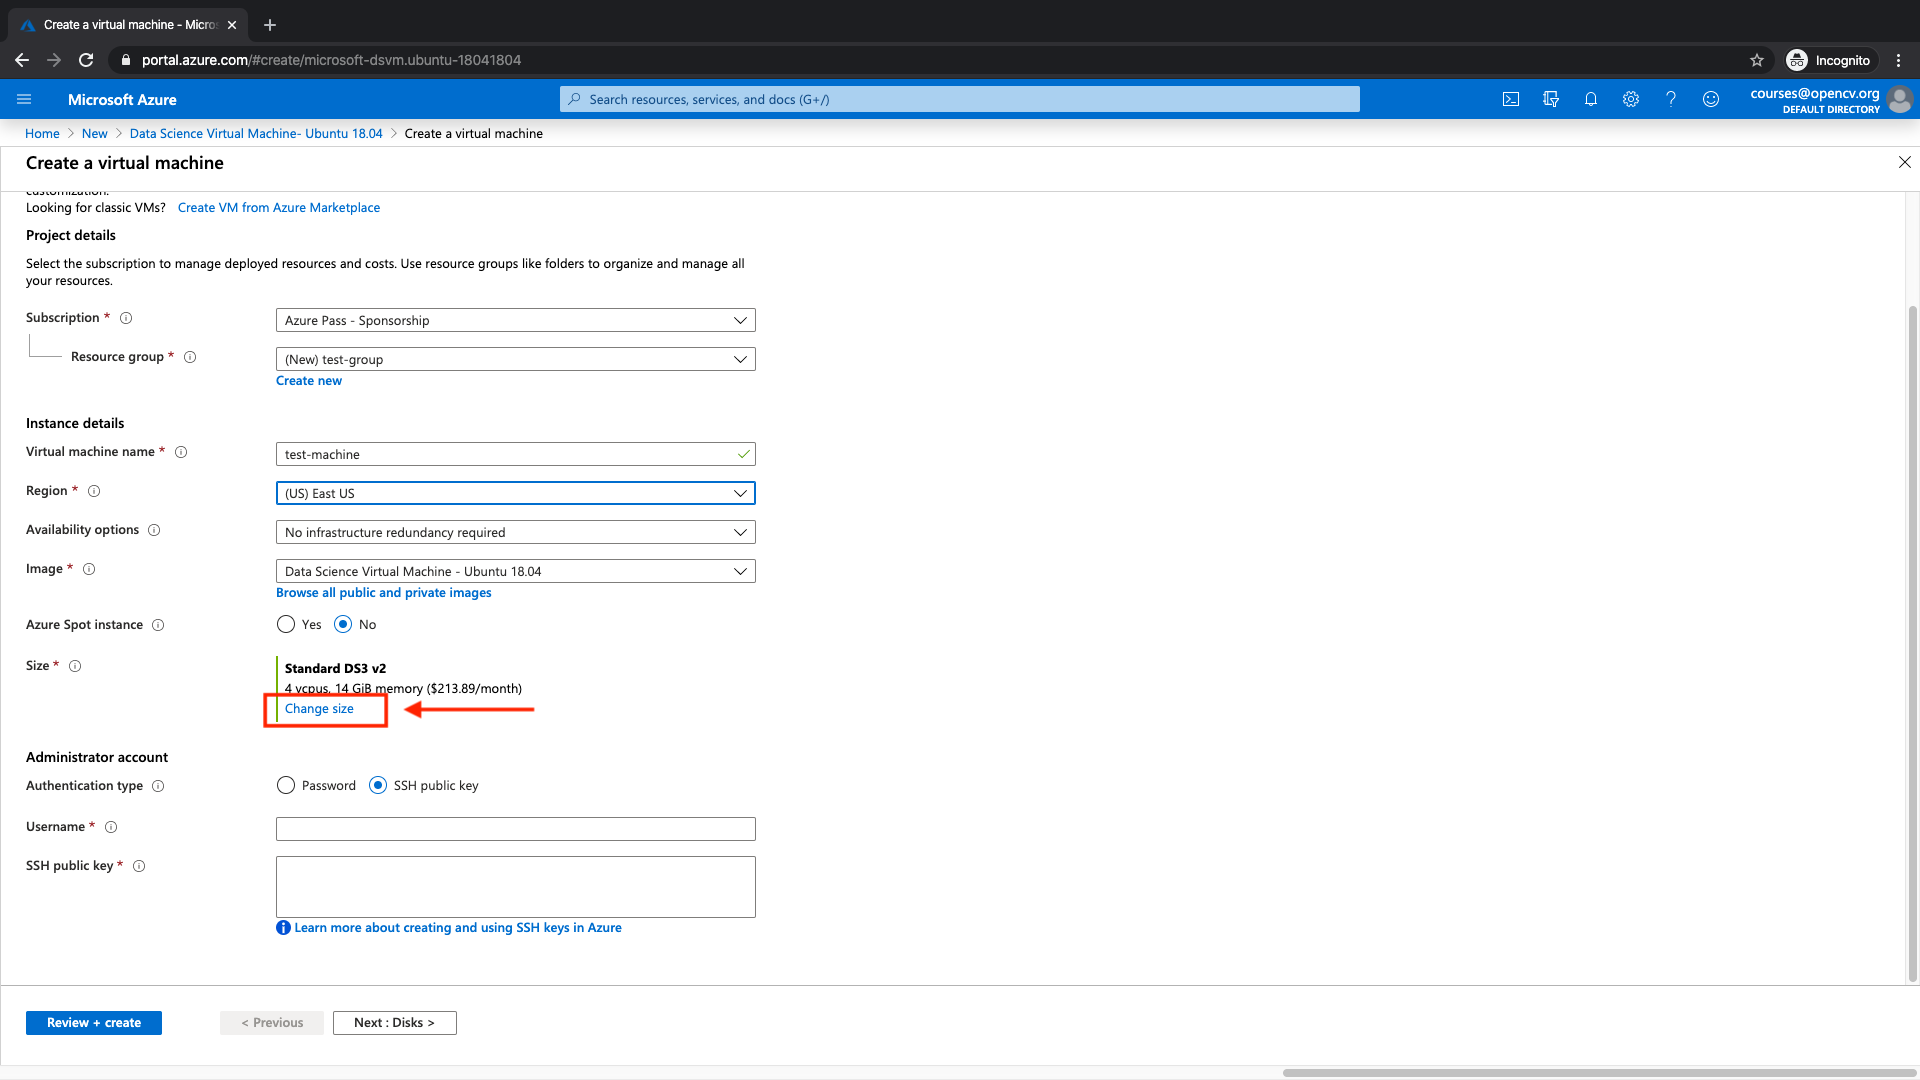
\includegraphics[scale=0.20]{figures/vm8}
%\caption{\small \sl . \cite{Mallick m.fl. 2020} \label{fig:azure}}
\end{center}
\end{figure}

\begin{figure}[H]
\begin{center} 
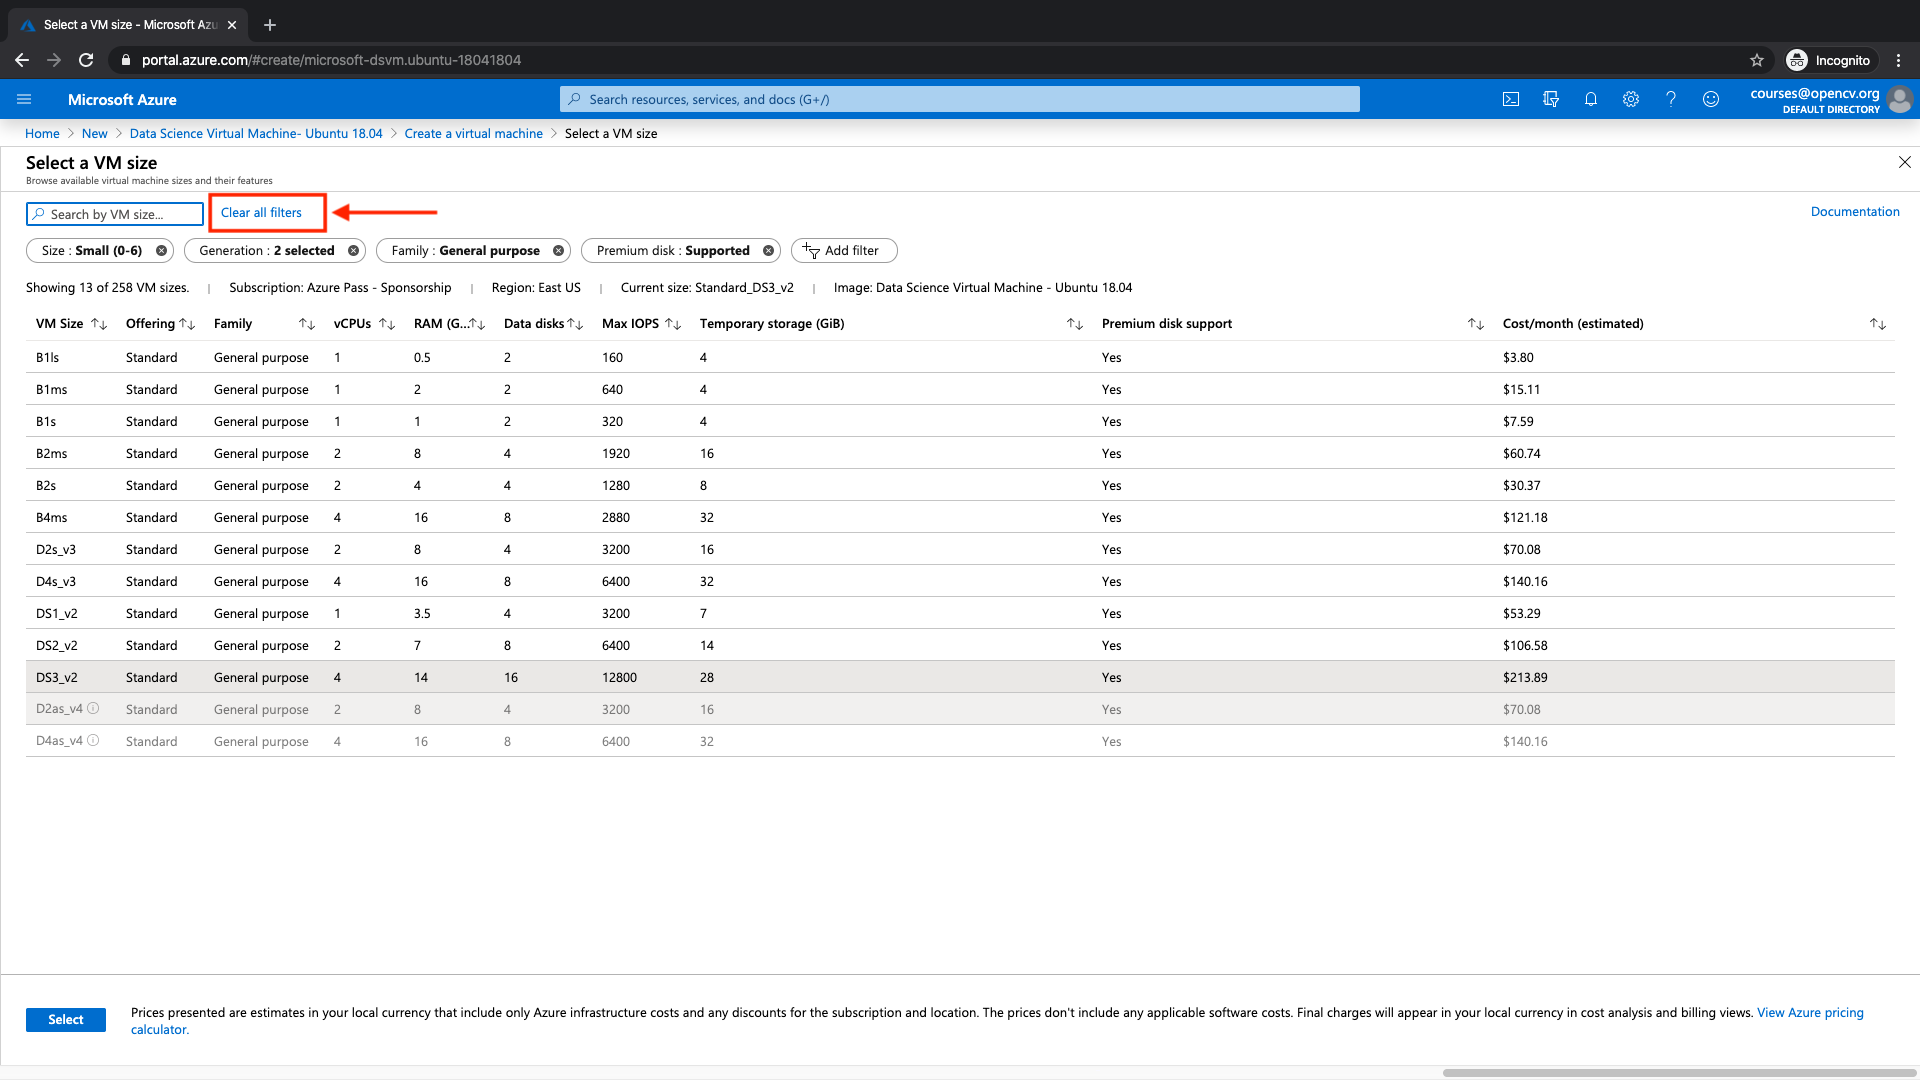
\includegraphics[scale=0.20]{figures/vm9}
%\caption{\small \sl . \cite{Mallick m.fl. 2020} \label{fig:azure}}
\end{center}
\end{figure}

\begin{figure}[H]
\begin{center} 
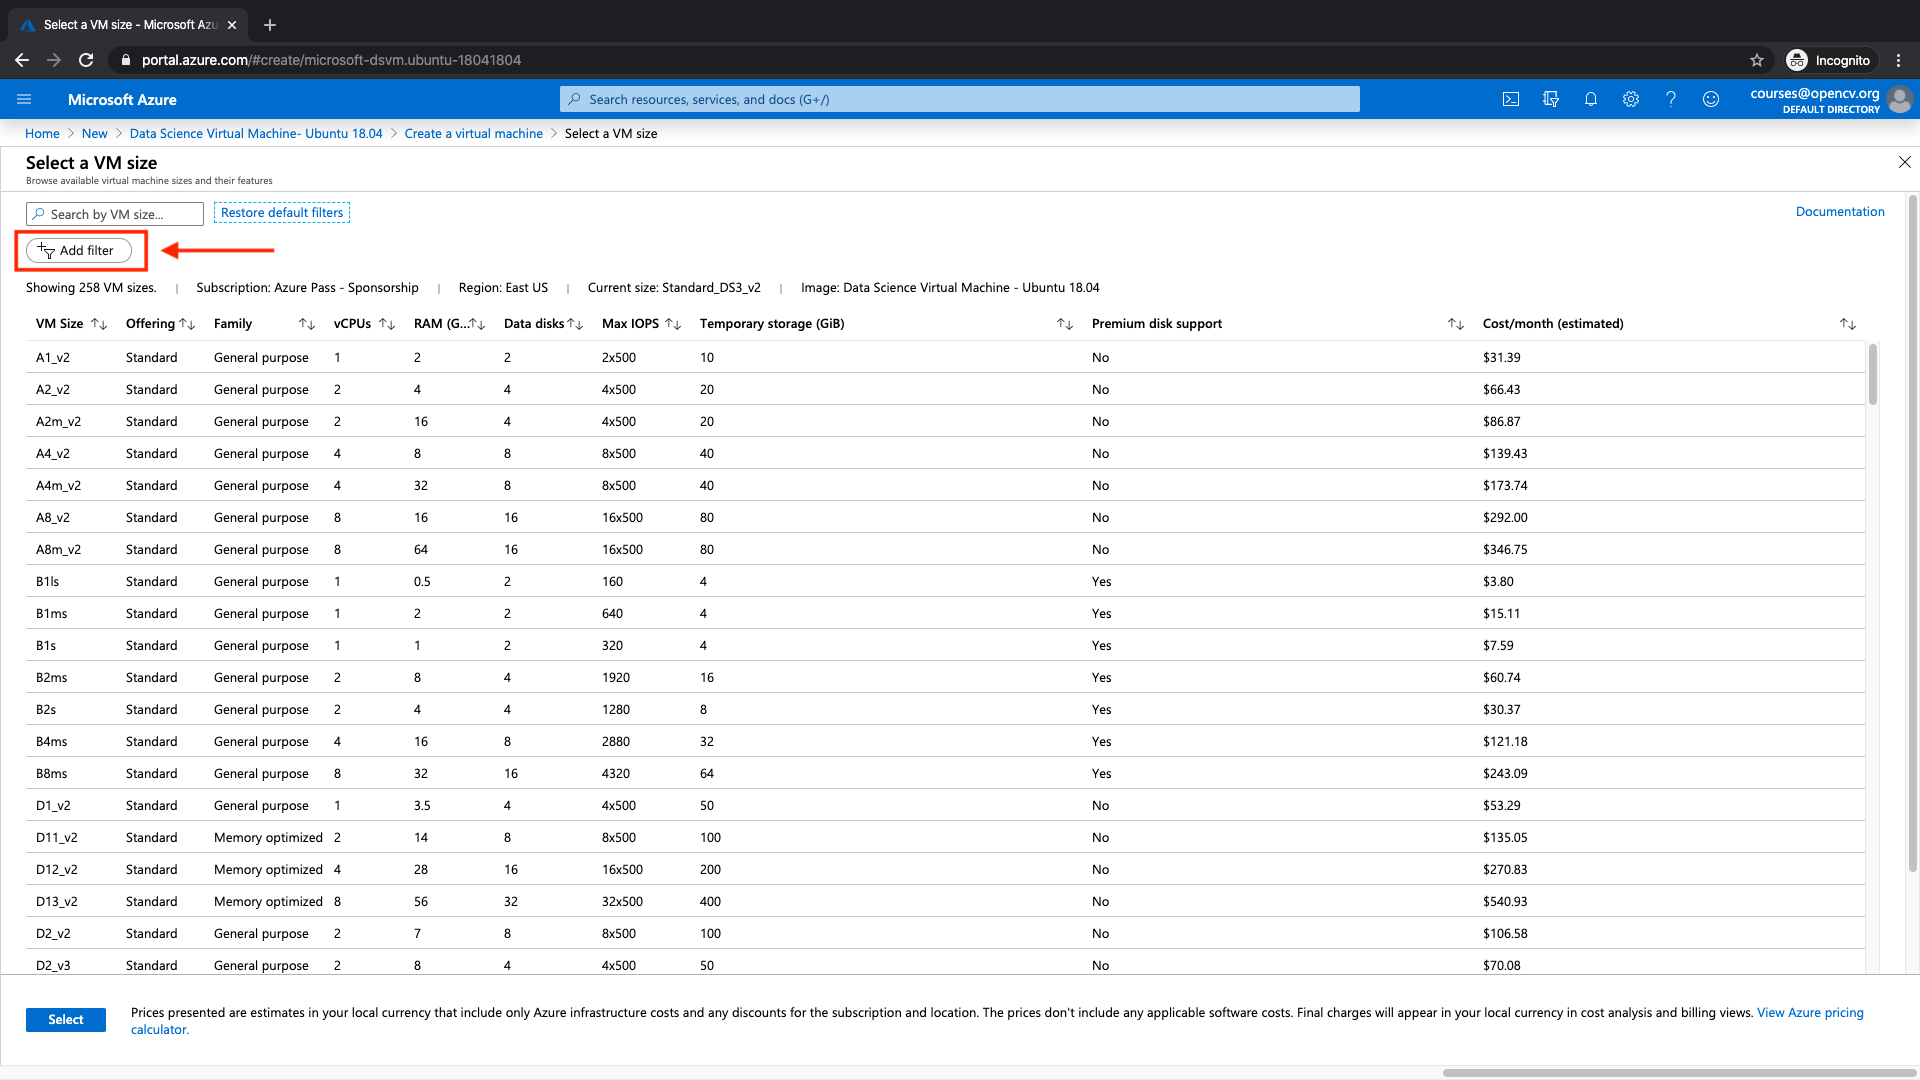
\includegraphics[scale=0.20]{figures/vm10}
%\caption{\small \sl . \cite{Mallick m.fl. 2020} \label{fig:azure}}
\end{center}
\end{figure}

11. Select the NC6\_Promo instance
You can see the information about the instance, for example it is from the GPU family and has 6 vCPUs, 56GB of RAM, storage of 380GB and the price is 289 dollar.

\begin{figure}[H]
\begin{center} 
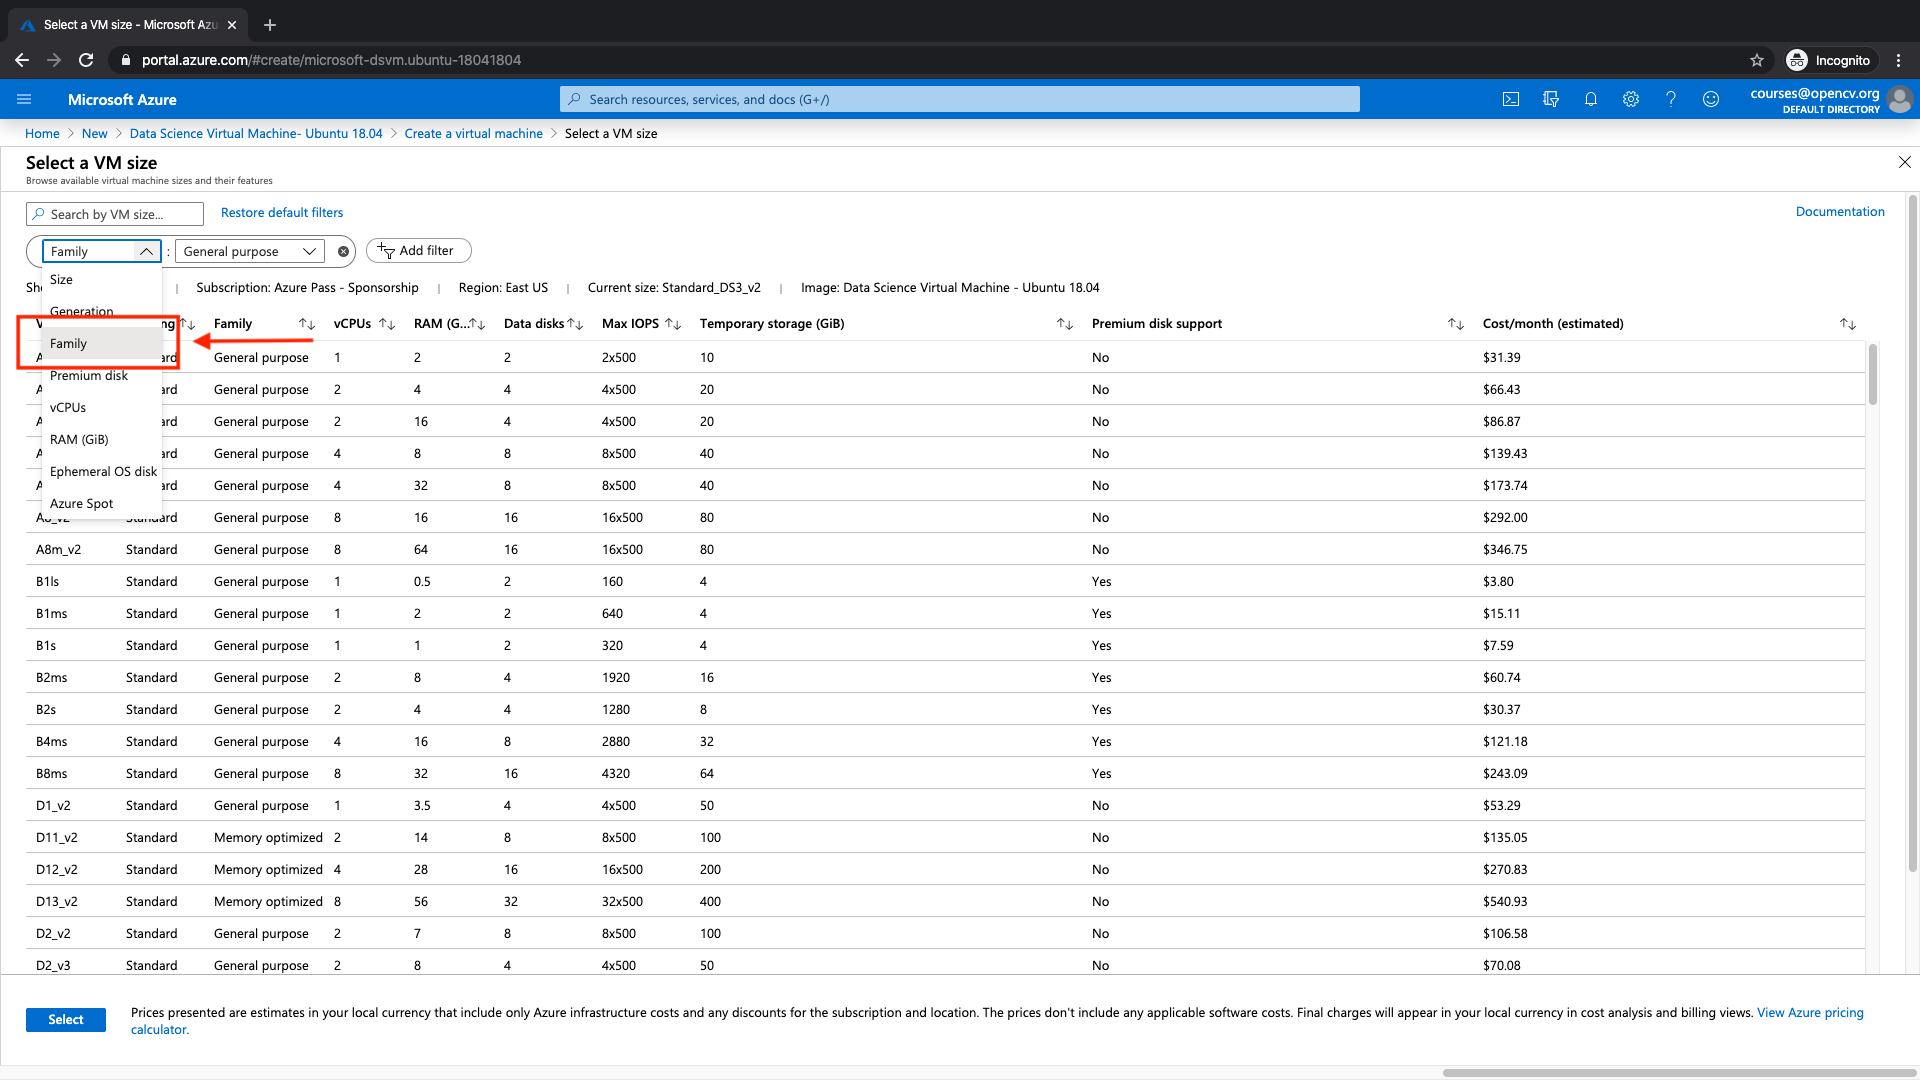
\includegraphics[scale=0.20]{figures/vm11}
%\caption{\small \sl . \cite{Mallick m.fl. 2020} \label{fig:azure}}
\end{center}
\end{figure}

\begin{figure}[H]
\begin{center} 
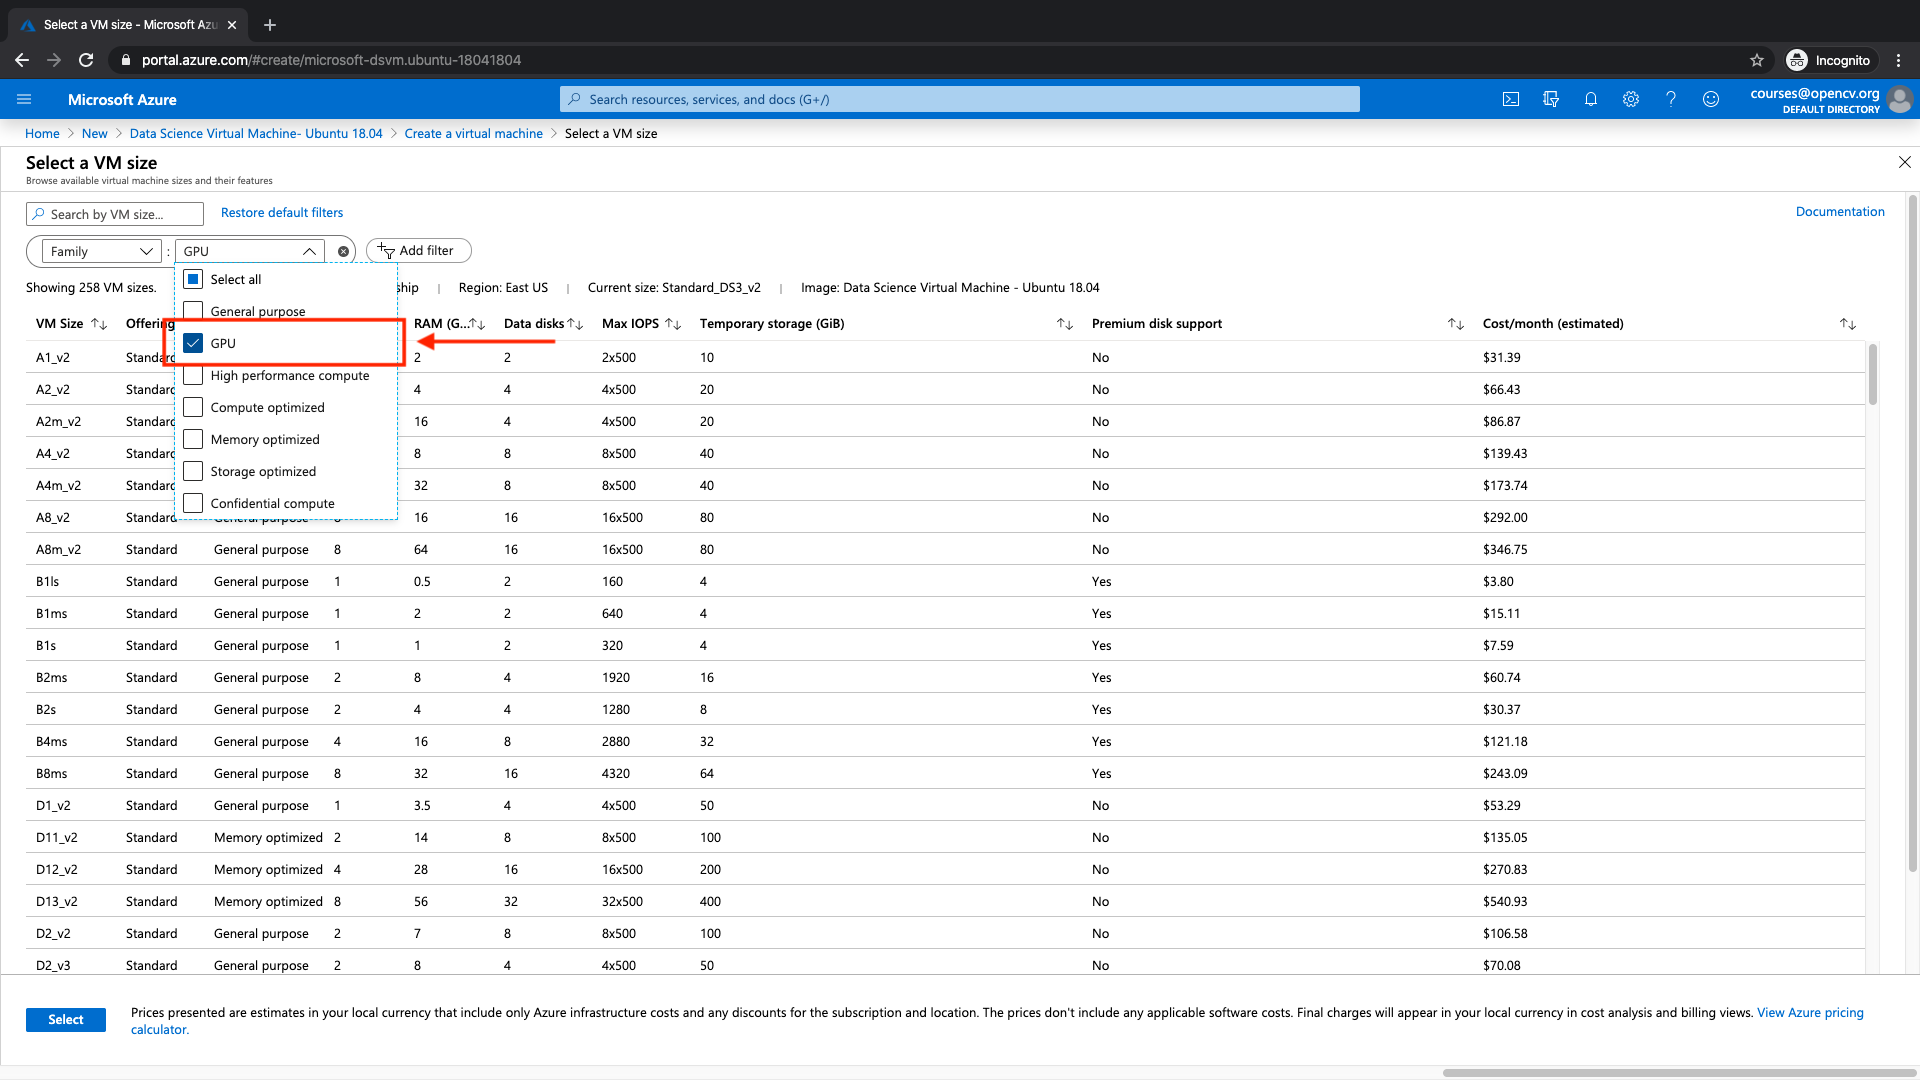
\includegraphics[scale=0.20]{figures/vm12}
%\caption{\small \sl . \cite{Mallick m.fl. 2020} \label{fig:azure}}
\end{center}
\end{figure}

12. Check the updated instance
Check if the instance has changed according to your selection.

\begin{figure}[H]
\begin{center} 
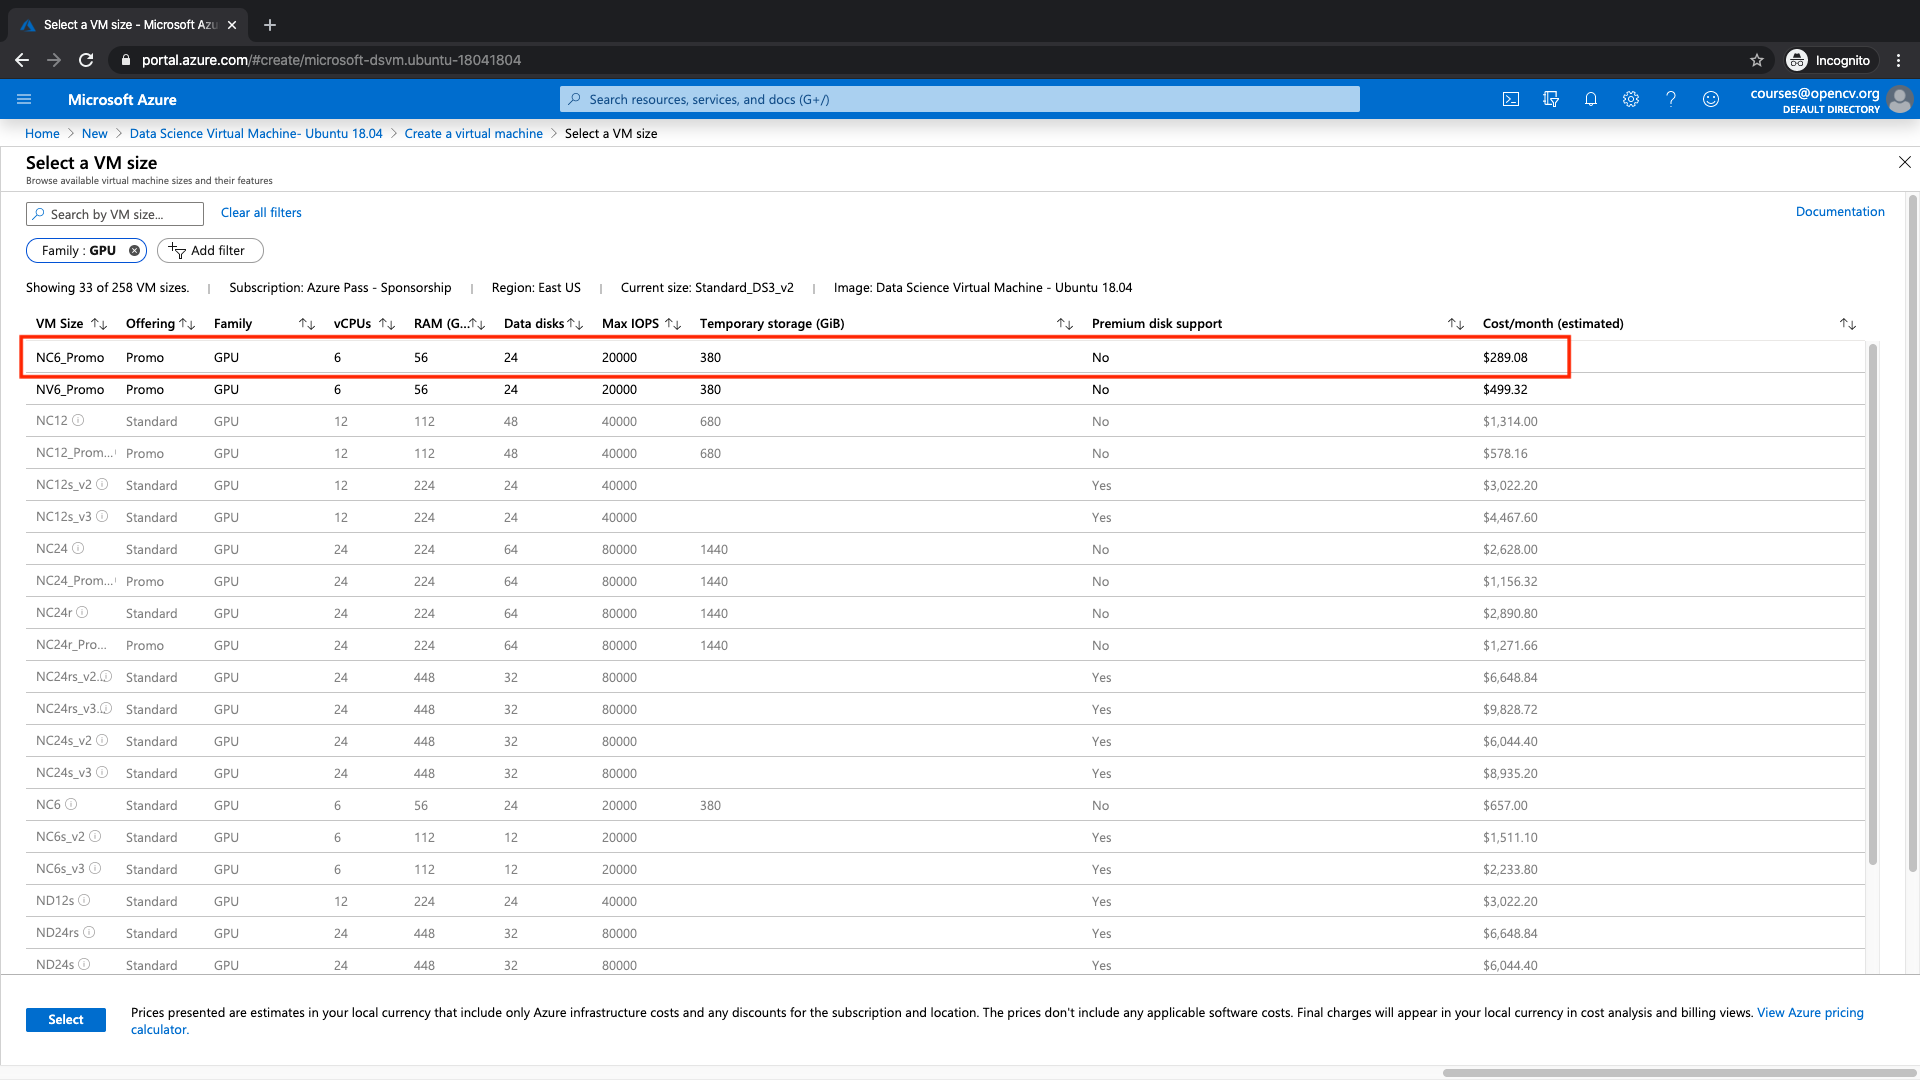
\includegraphics[scale=0.20]{figures/vm13}
%\caption{\small \sl . \cite{Mallick m.fl. 2020} \label{fig:azure}}
\end{center}
\end{figure}

13. Set up username and Password
For logging into the system, you can use ssh. But for using jupyter Notebooks directly, you need to set a username and password. These credentials can be used while logging in to the system as well as accessing jupyter notebooks as we will see later.

\begin{figure}[H]
\begin{center} 
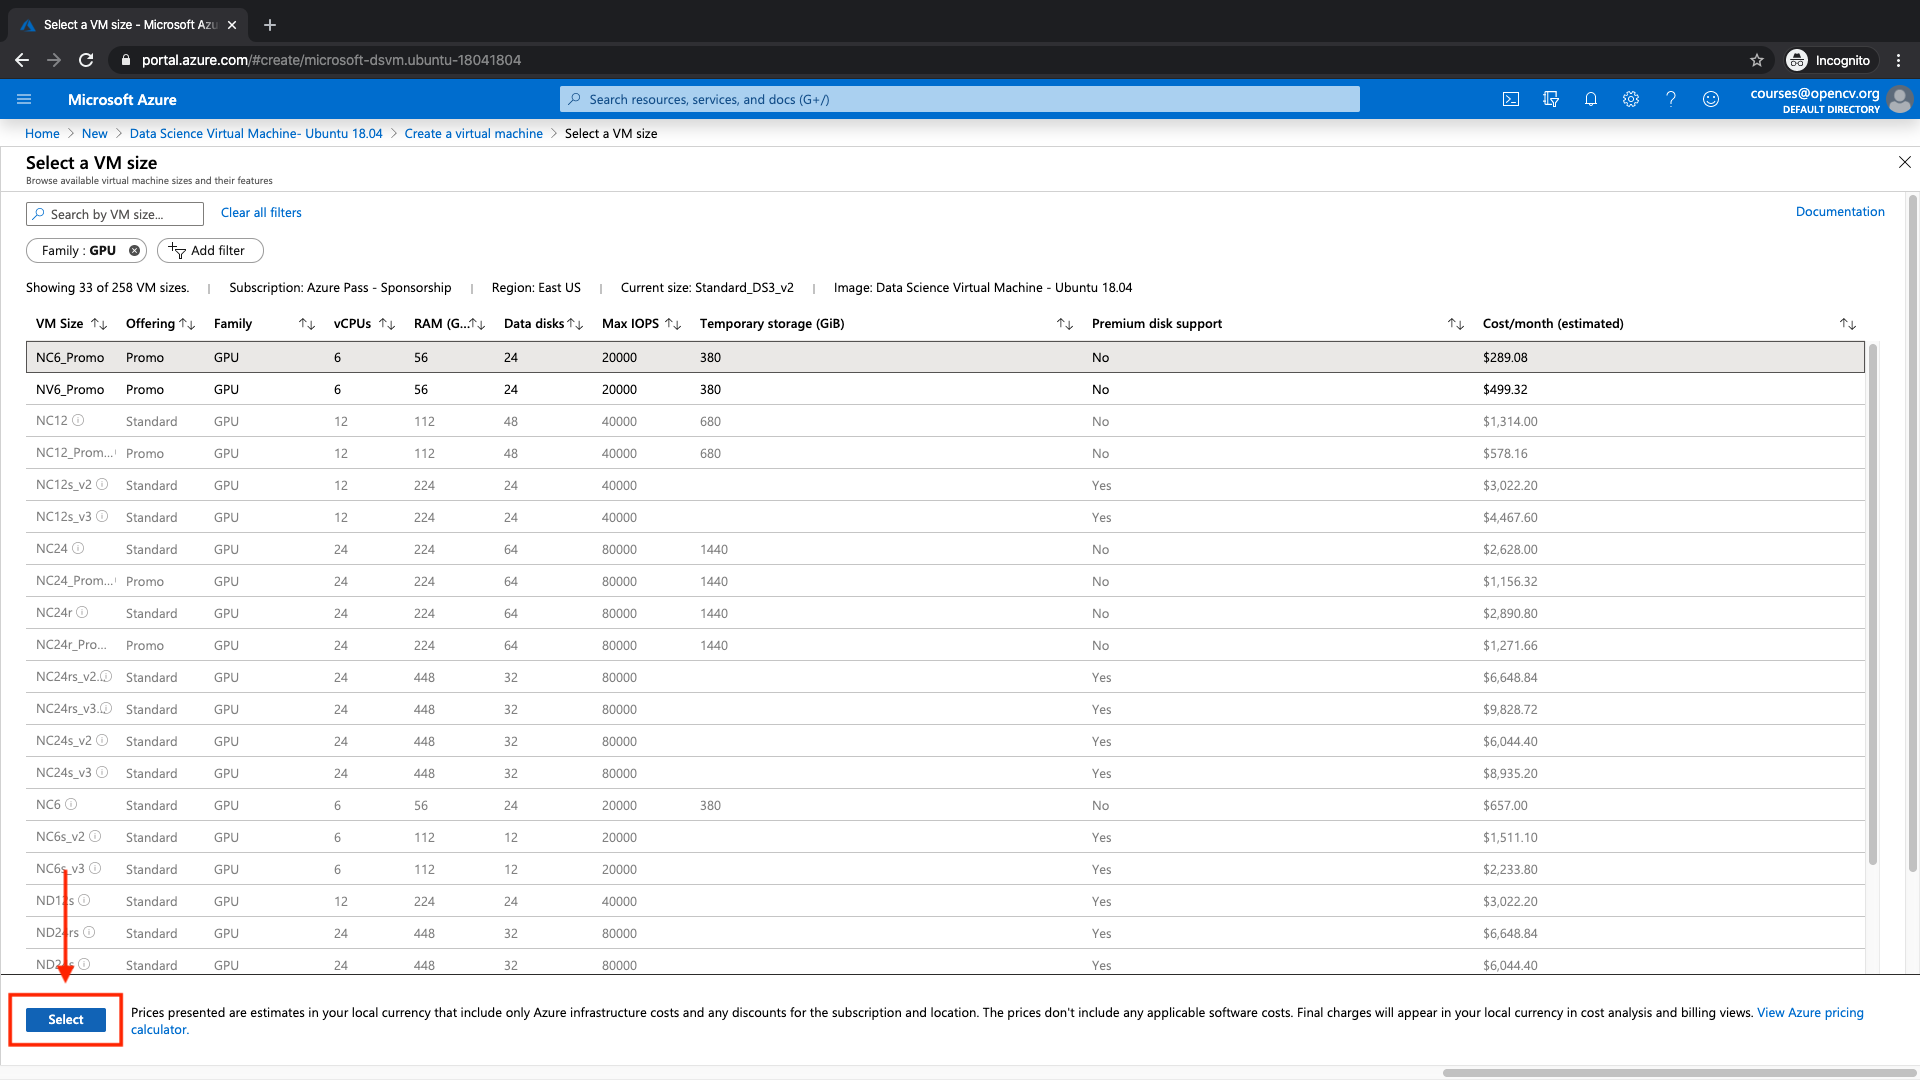
\includegraphics[scale=0.20]{figures/vm14}
%\caption{\small \sl . \cite{Mallick m.fl. 2020} \label{fig:azure}}
\end{center}
\end{figure}

14. Select Disks
We do not have to change anything here. If you want to add separate disks, then you have to edit this step accordingly.

\begin{figure}[H]
\begin{center} 
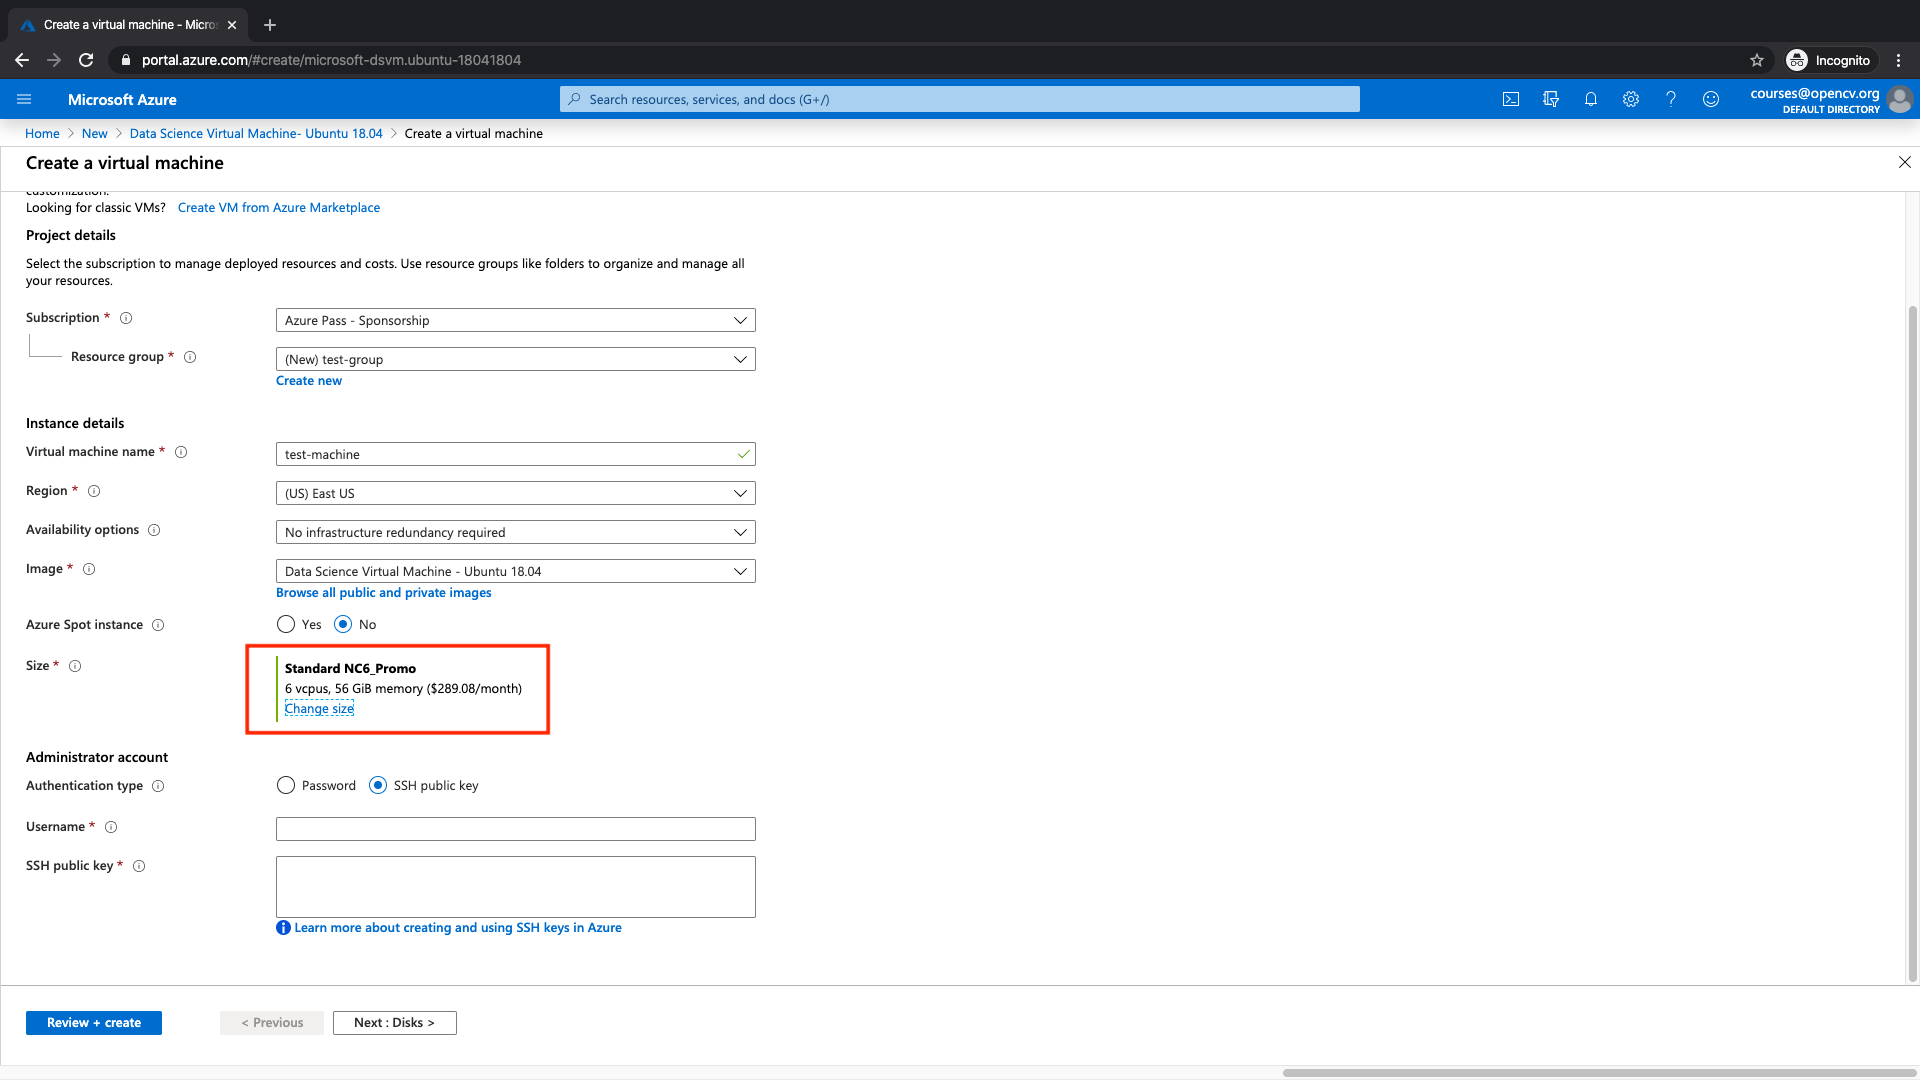
\includegraphics[scale=0.20]{figures/vm15}
%\caption{\small \sl . \cite{Mallick m.fl. 2020} \label{fig:azure}}
\end{center}
\end{figure}

15. Set up Networking
We just keep the defaults.

\begin{figure}[H]
\begin{center} 
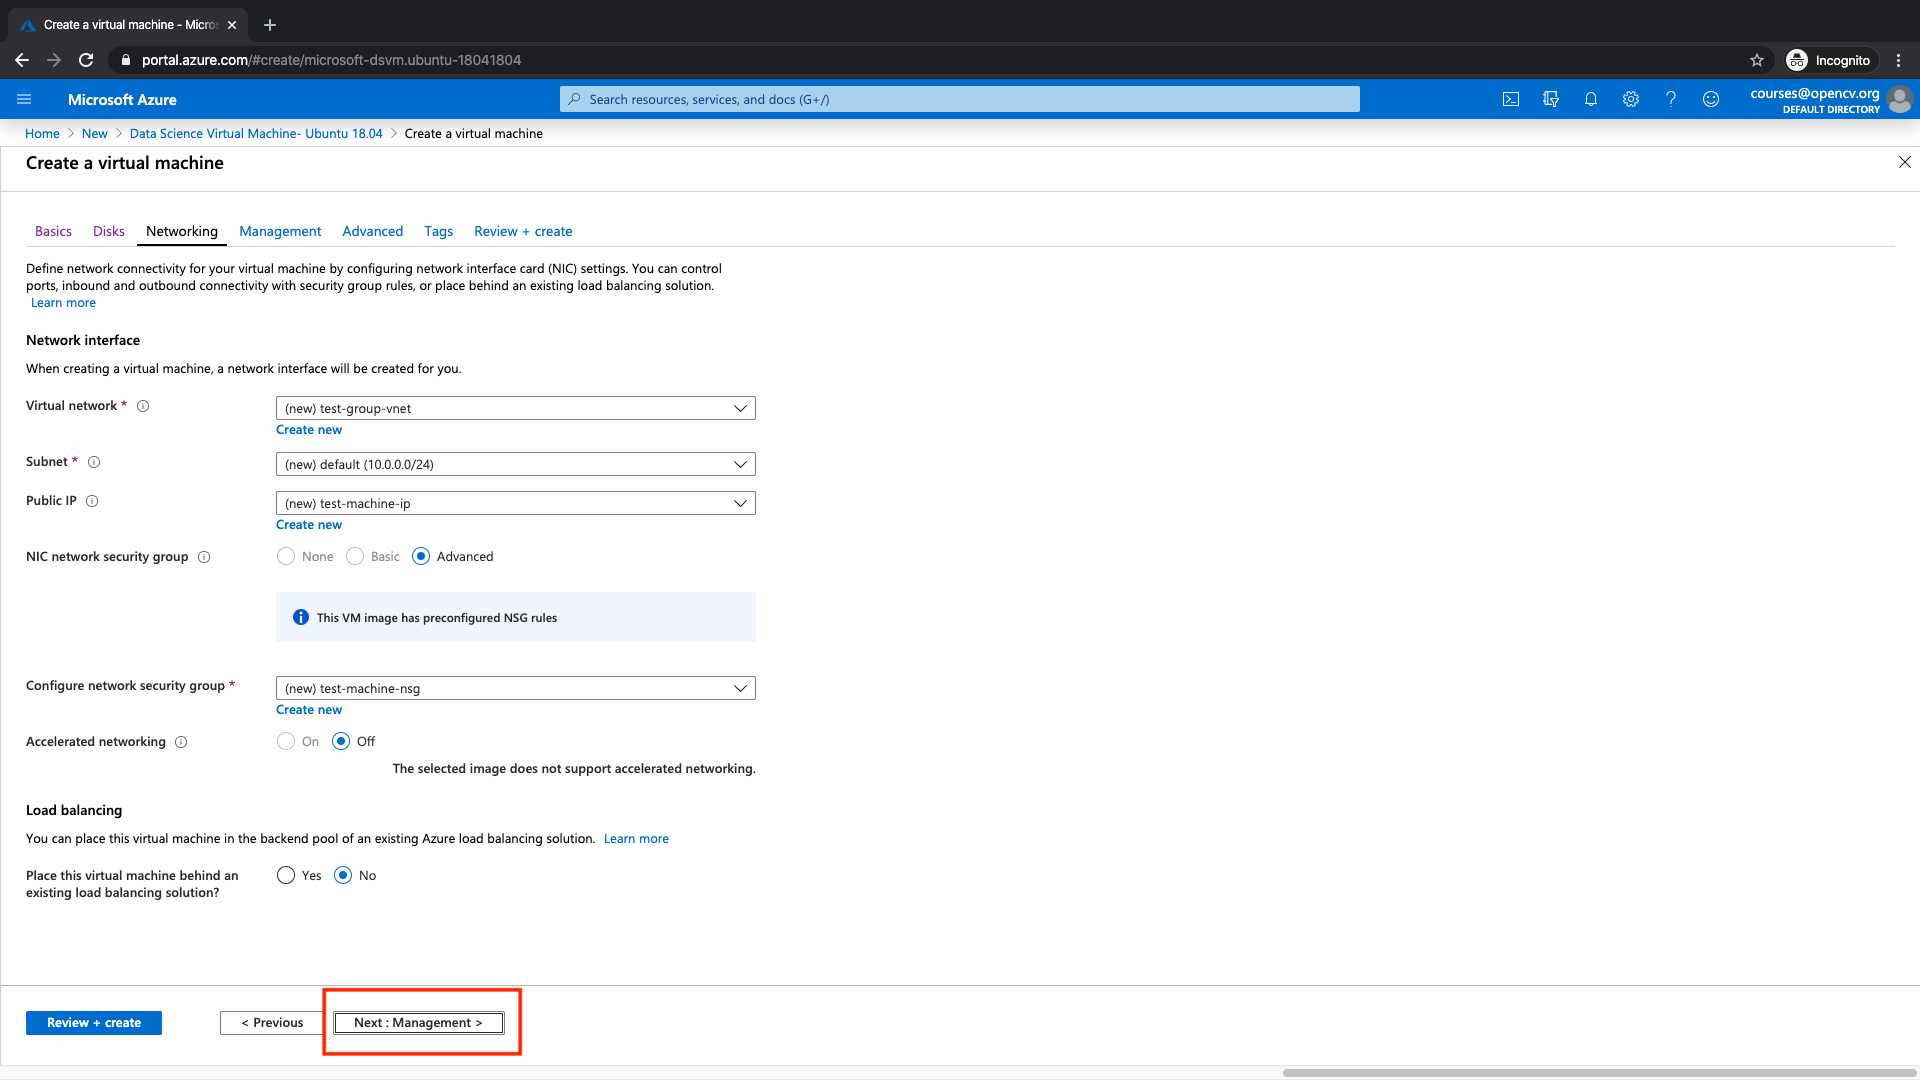
\includegraphics[scale=0.20]{figures/vm18}
%\caption{\small \sl . \cite{Mallick m.fl. 2020} \label{fig:azure}}
\end{center}
\end{figure}

16. Configure Management options
You need to specify management options here. Create a new storage account and click next as shown below.

\begin{figure}[H]
\begin{center} 
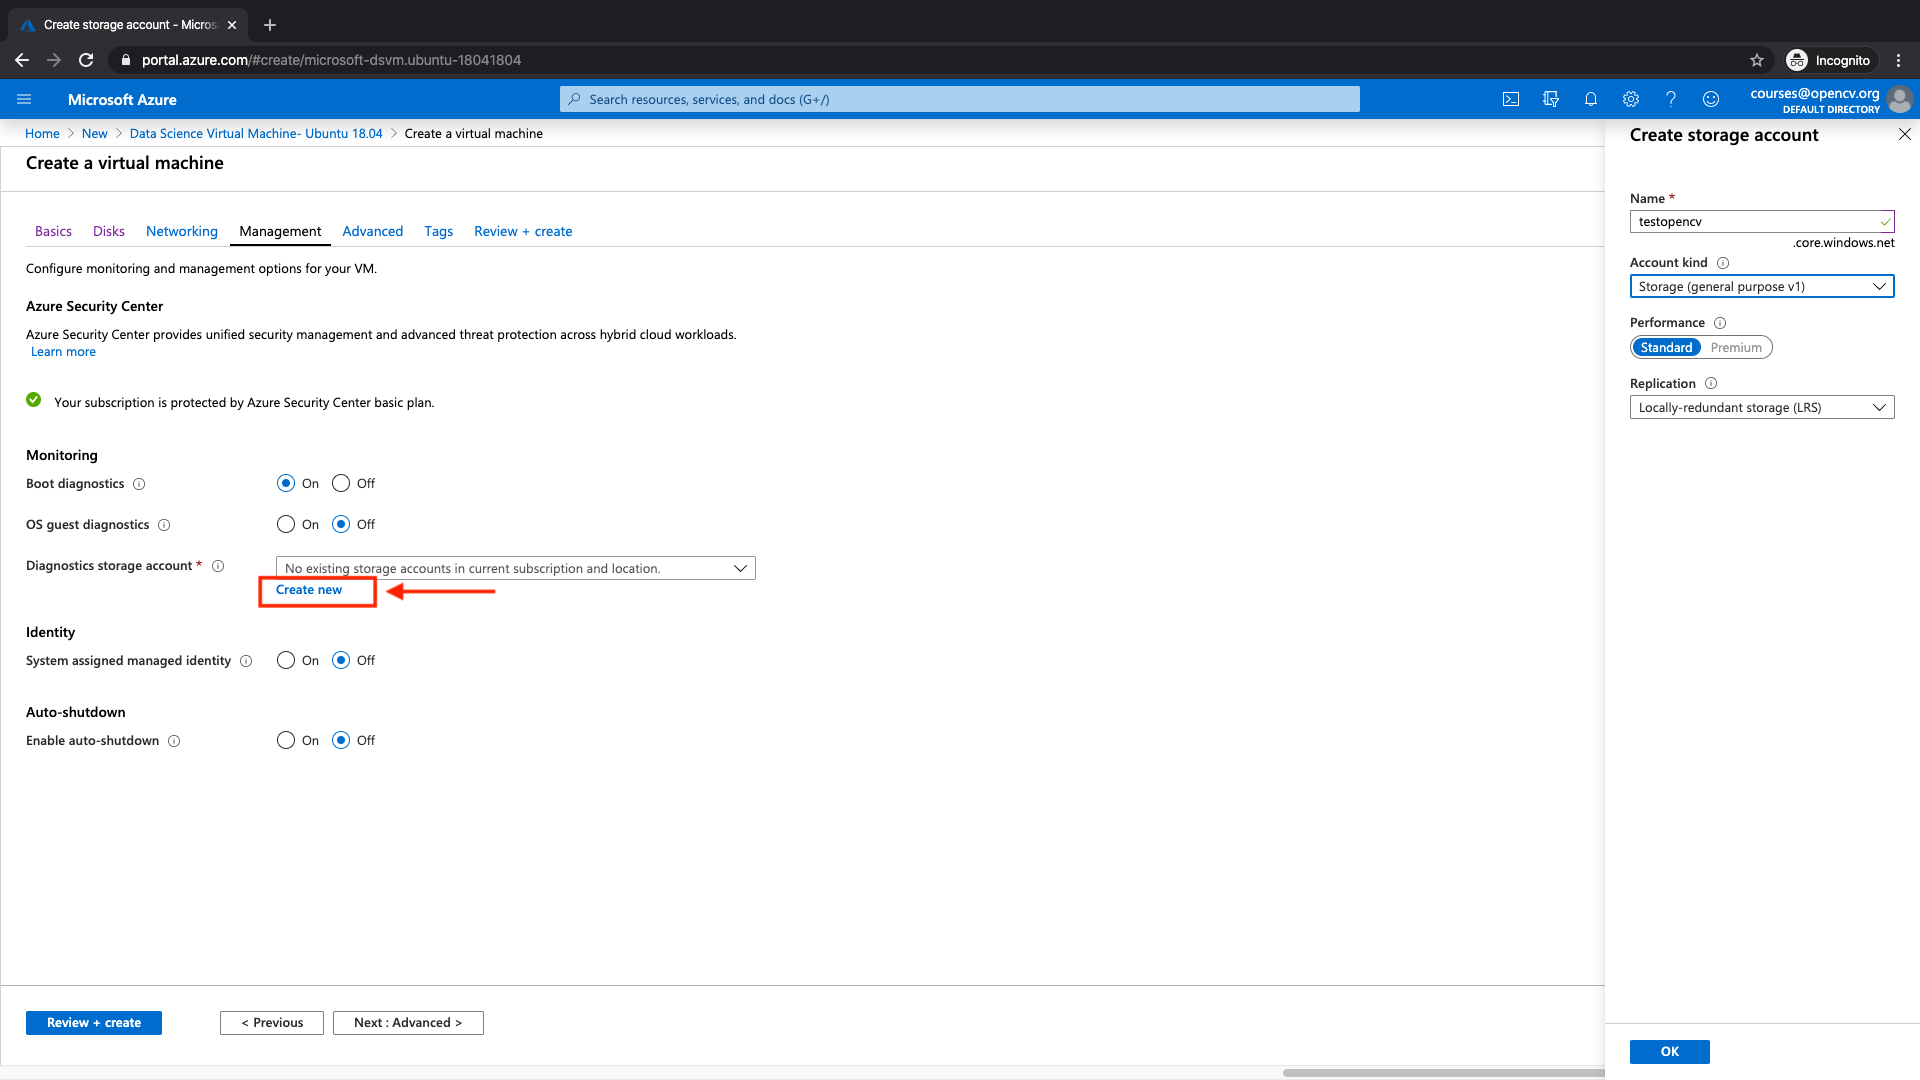
\includegraphics[scale=0.20]{figures/vm19}
%\caption{\small \sl . \cite{Mallick m.fl. 2020} \label{fig:azure}}
\end{center}
\end{figure}

\begin{figure}[H]
\begin{center} 
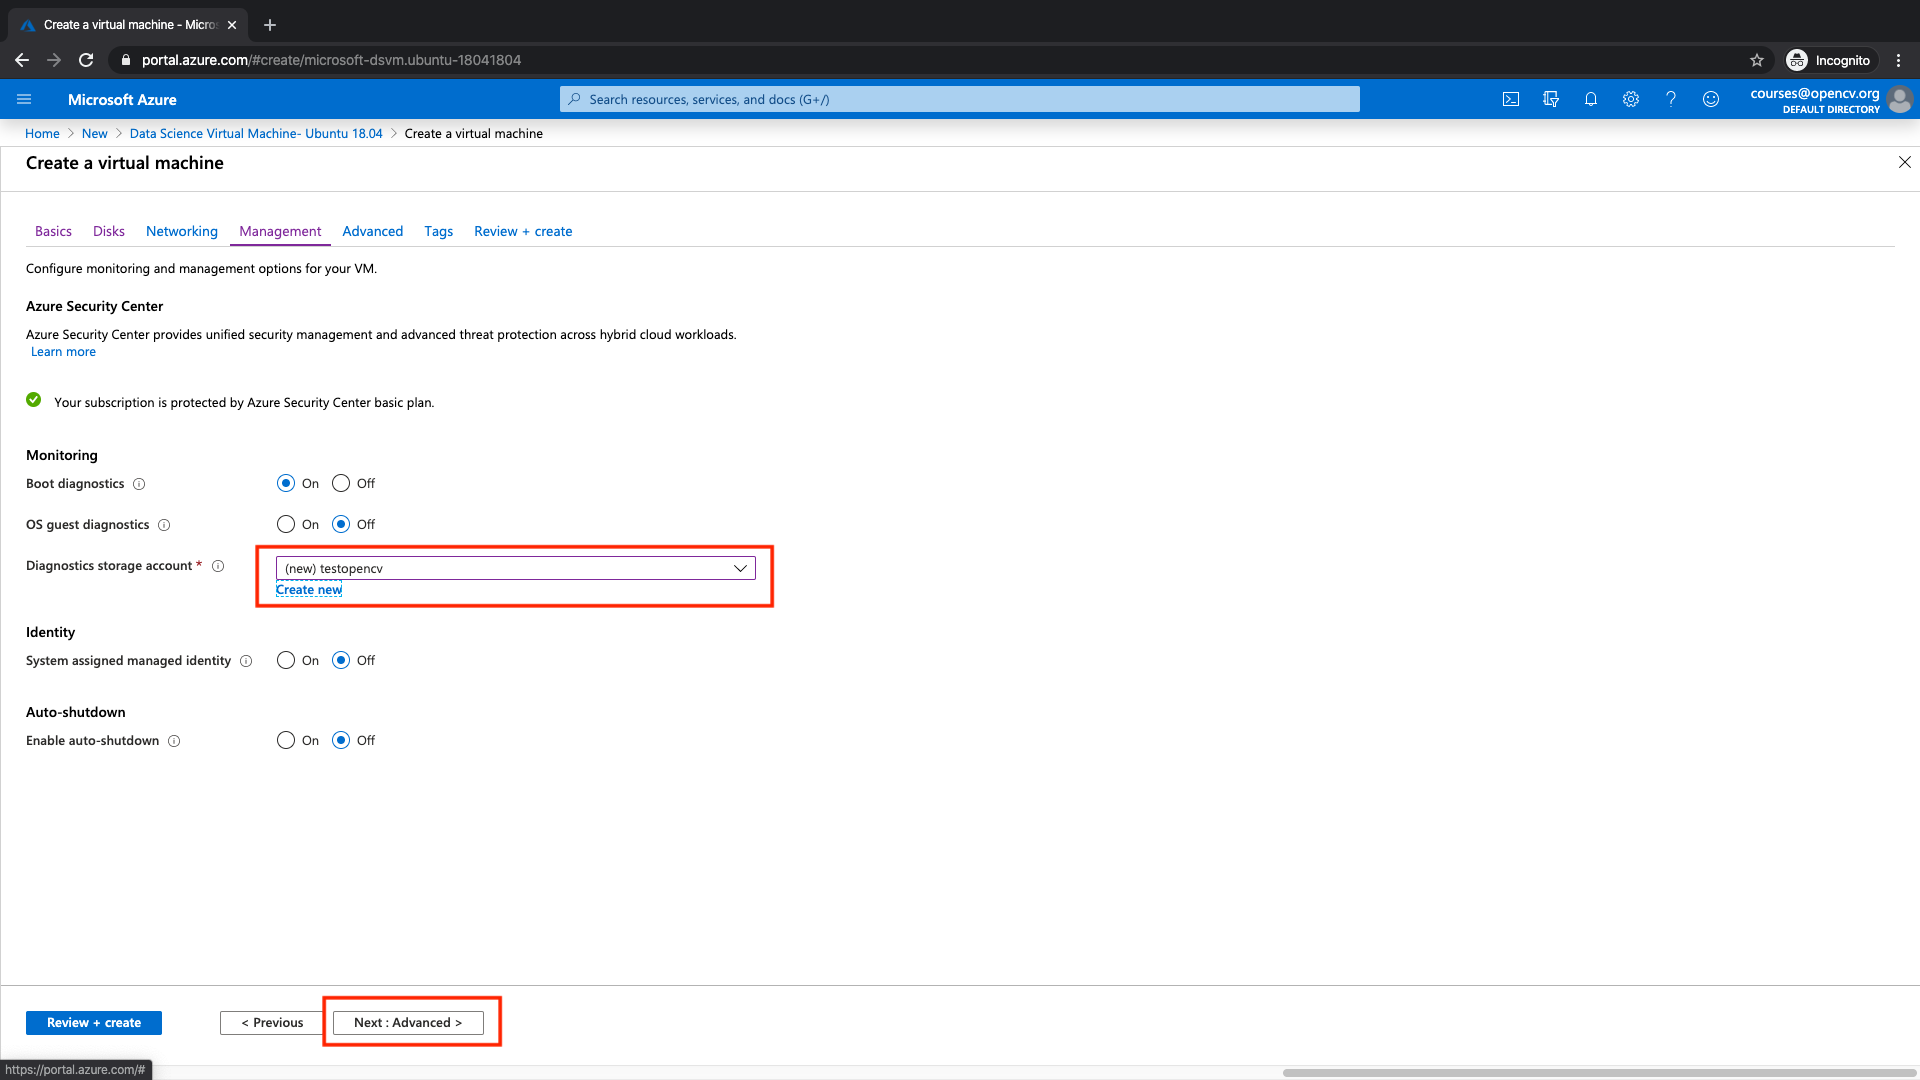
\includegraphics[scale=0.20]{figures/vm20}
%\caption{\small \sl . \cite{Mallick m.fl. 2020} \label{fig:azure}}
\end{center}
\end{figure}

17. Advanced options
We will keep the default options.

\begin{figure}[H]
\begin{center} 
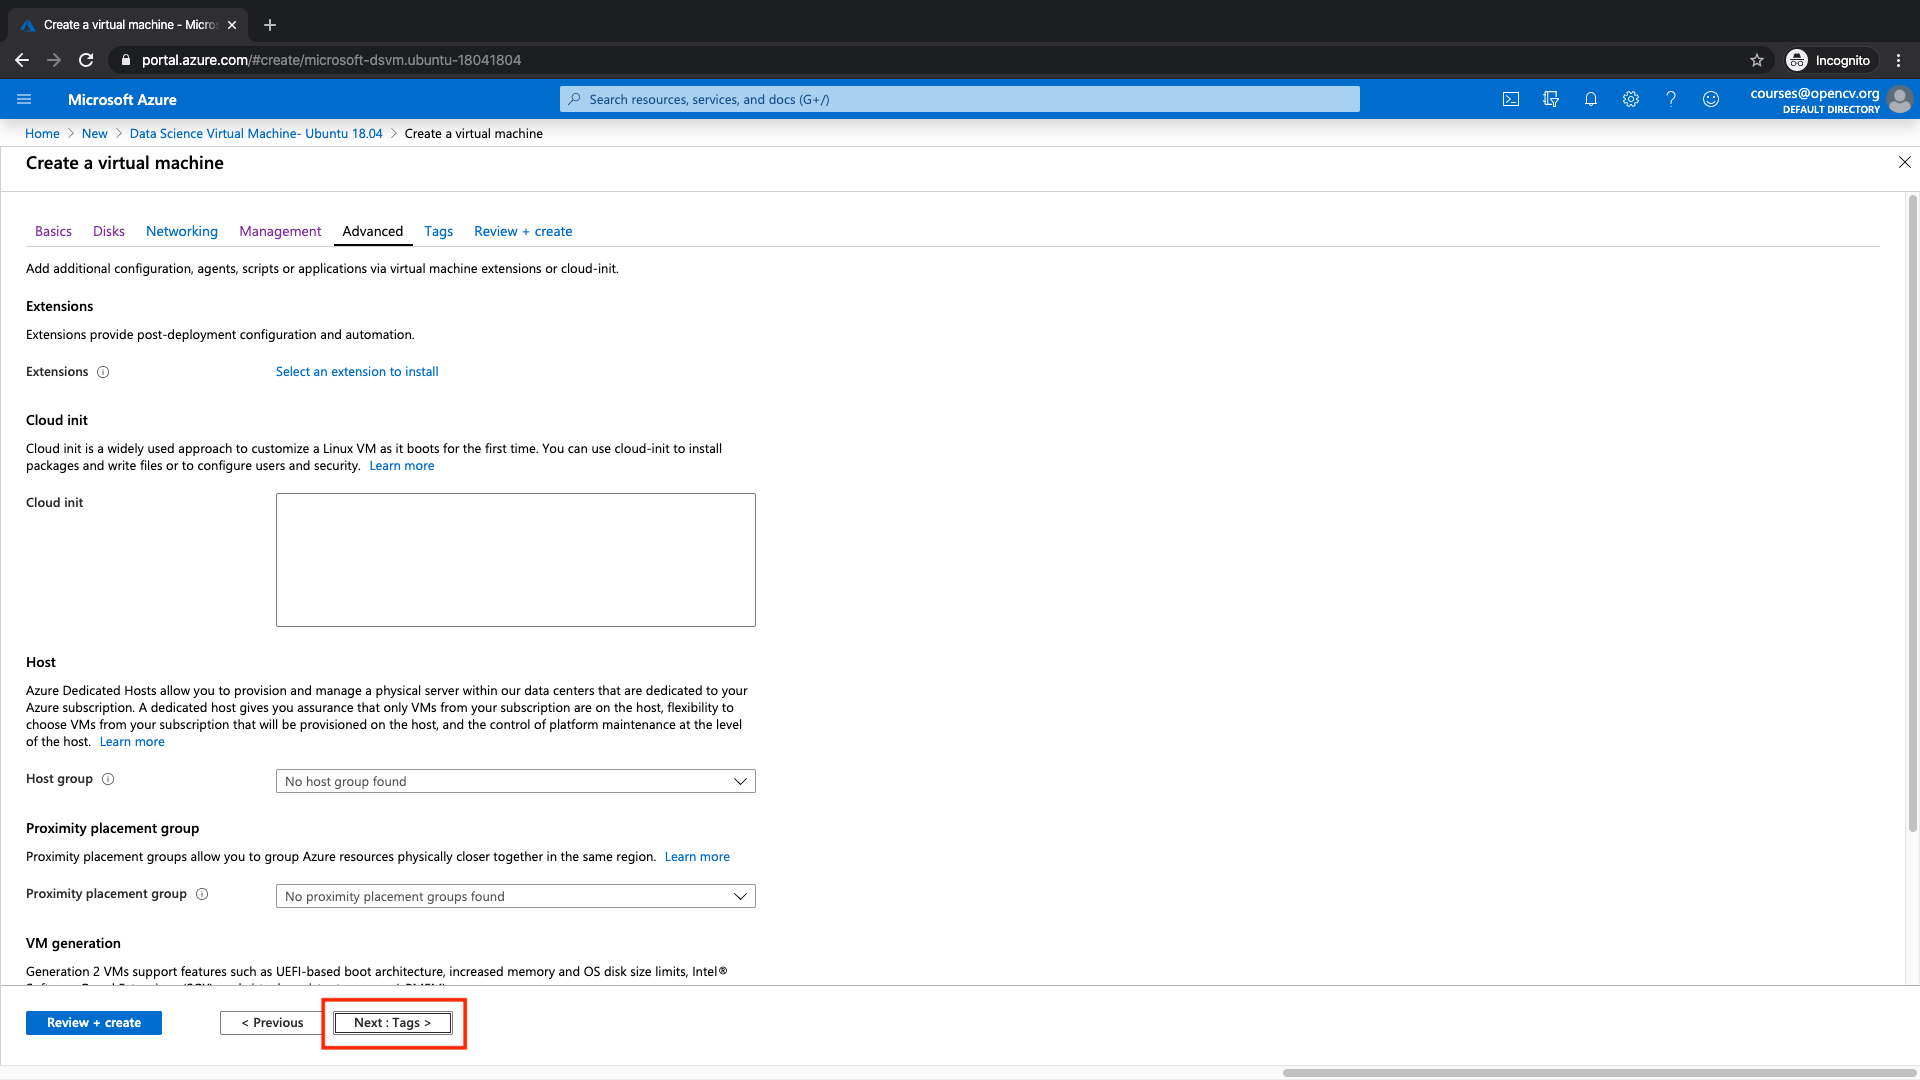
\includegraphics[scale=0.20]{figures/vm21}
%\caption{\small \sl . \cite{Mallick m.fl. 2020} \label{fig:azure}}
\end{center}
\end{figure}

18. Add tags
You can add tags to your instances. It is a good practice since you may forget the purpose of each instance when you are dealing with multiple instances. We will add a Name tag so that we know this instance by a name!

\begin{figure}[H]
\begin{center} 
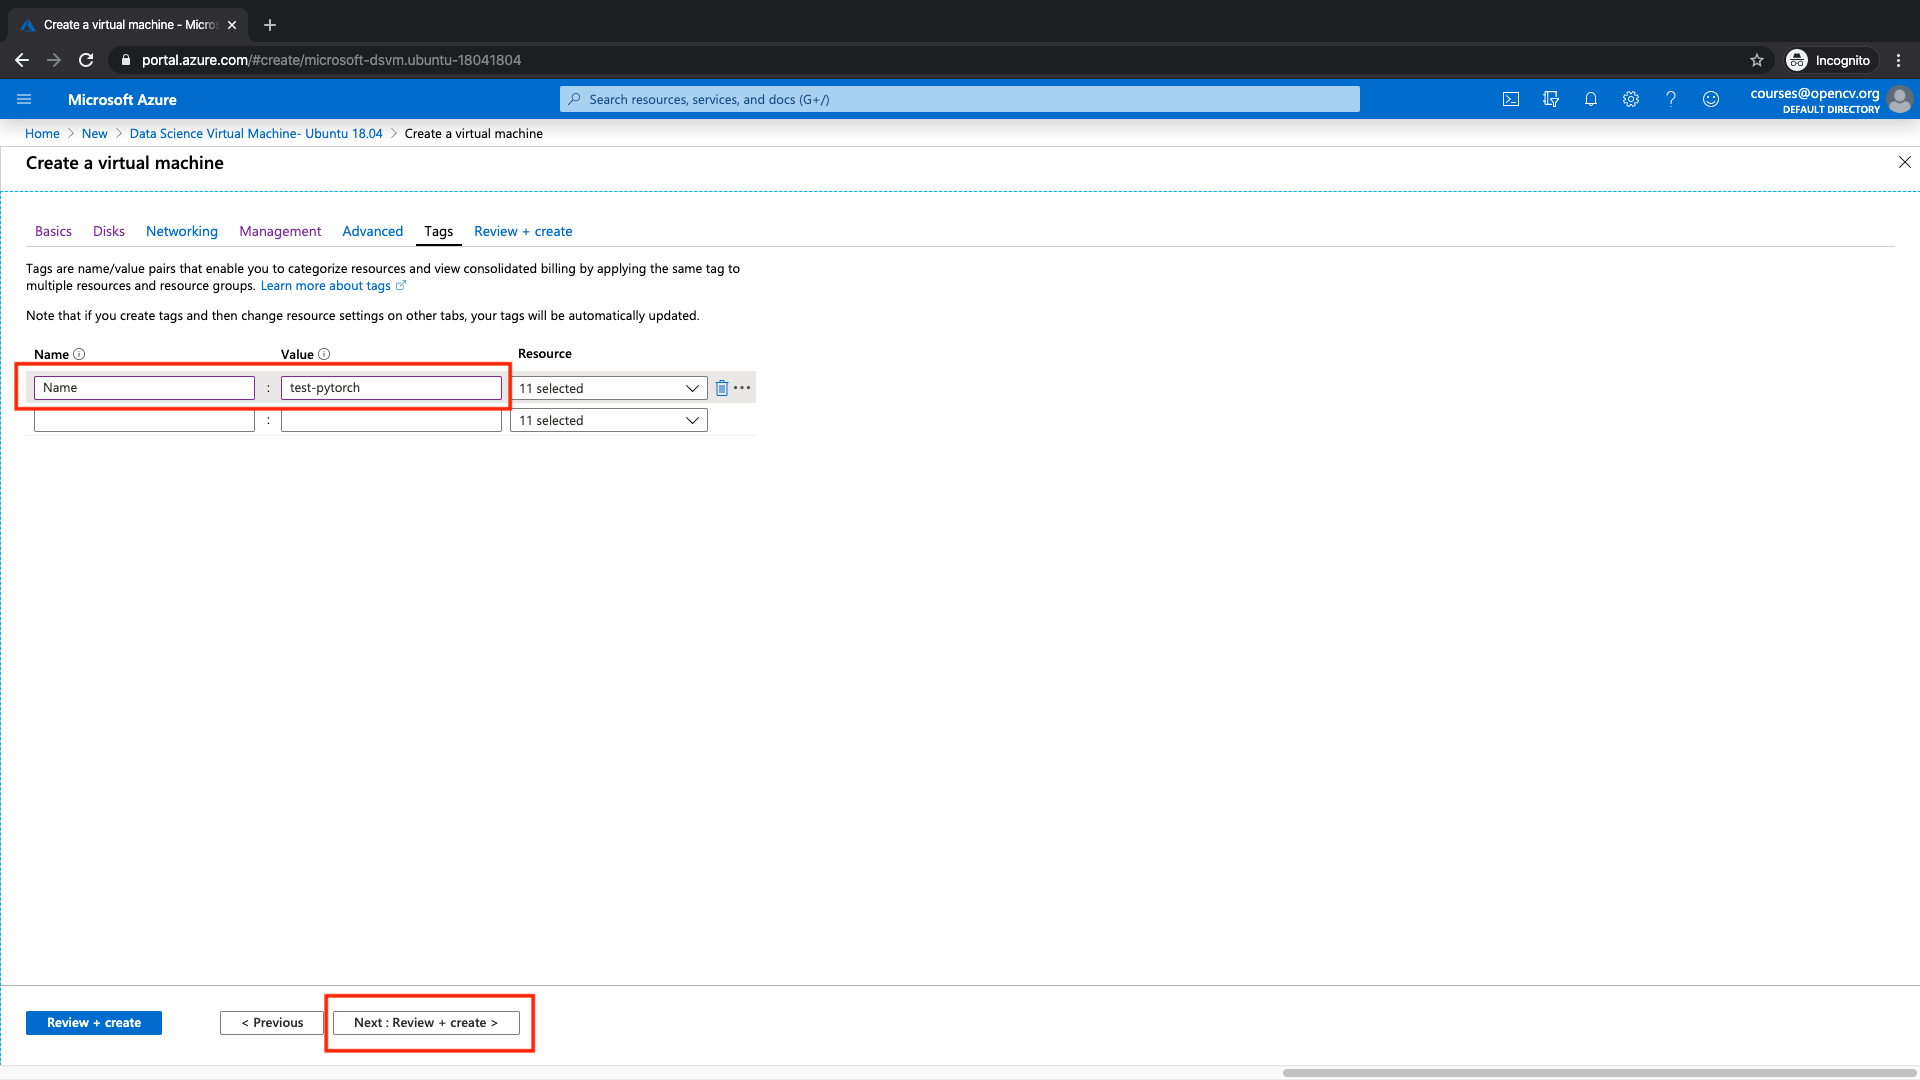
\includegraphics[scale=0.20]{figures/vm22}
%\caption{\small \sl . \cite{Mallick m.fl. 2020} \label{fig:azure}}
\end{center}
\end{figure}

19. Finish Configuration
We are done with the configuration steps and now we can create the instance. Click on Create

\begin{figure}[H]
\begin{center} 
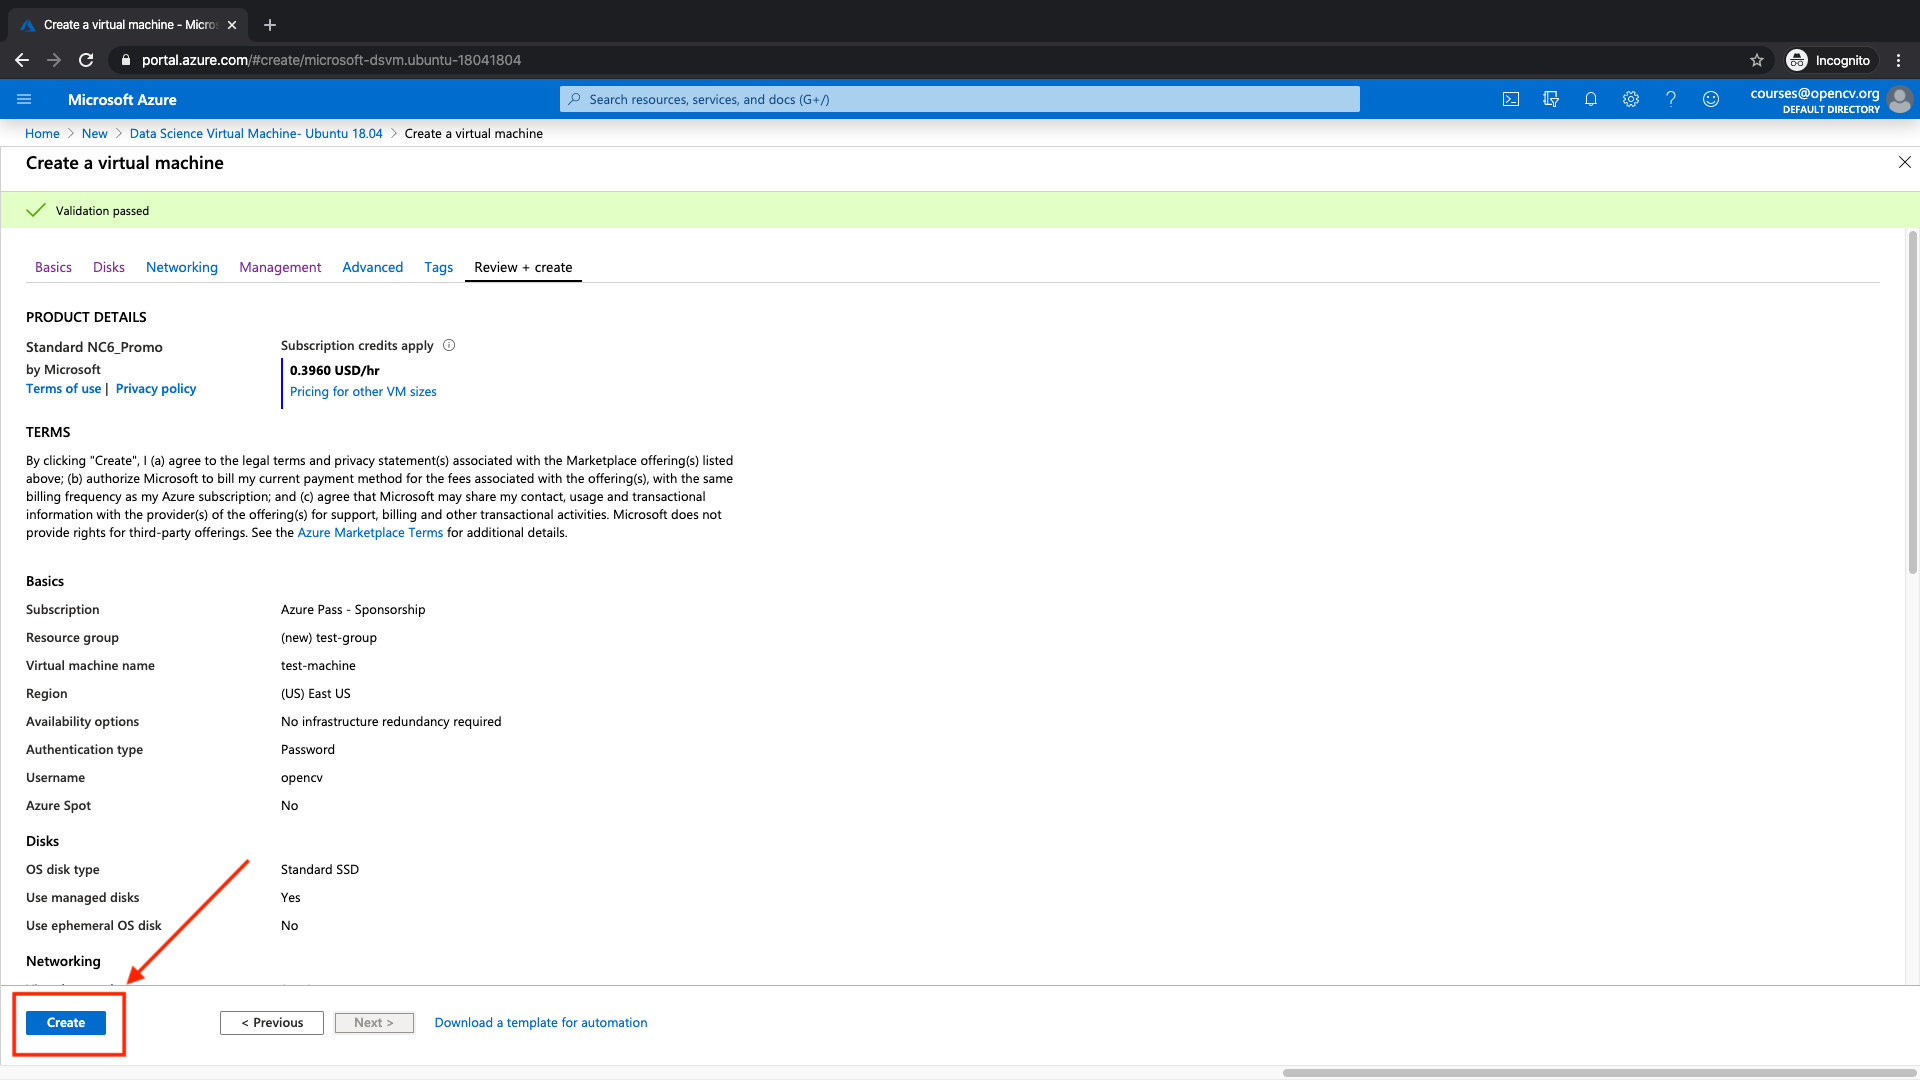
\includegraphics[scale=0.20]{figures/vm23}
%\caption{\small \sl . \cite{Mallick m.fl. 2020} \label{fig:azure}}
\end{center}
\end{figure}

This might take some time. . . ( 5 to 10 minutes )

\begin{figure}[H]
\begin{center} 
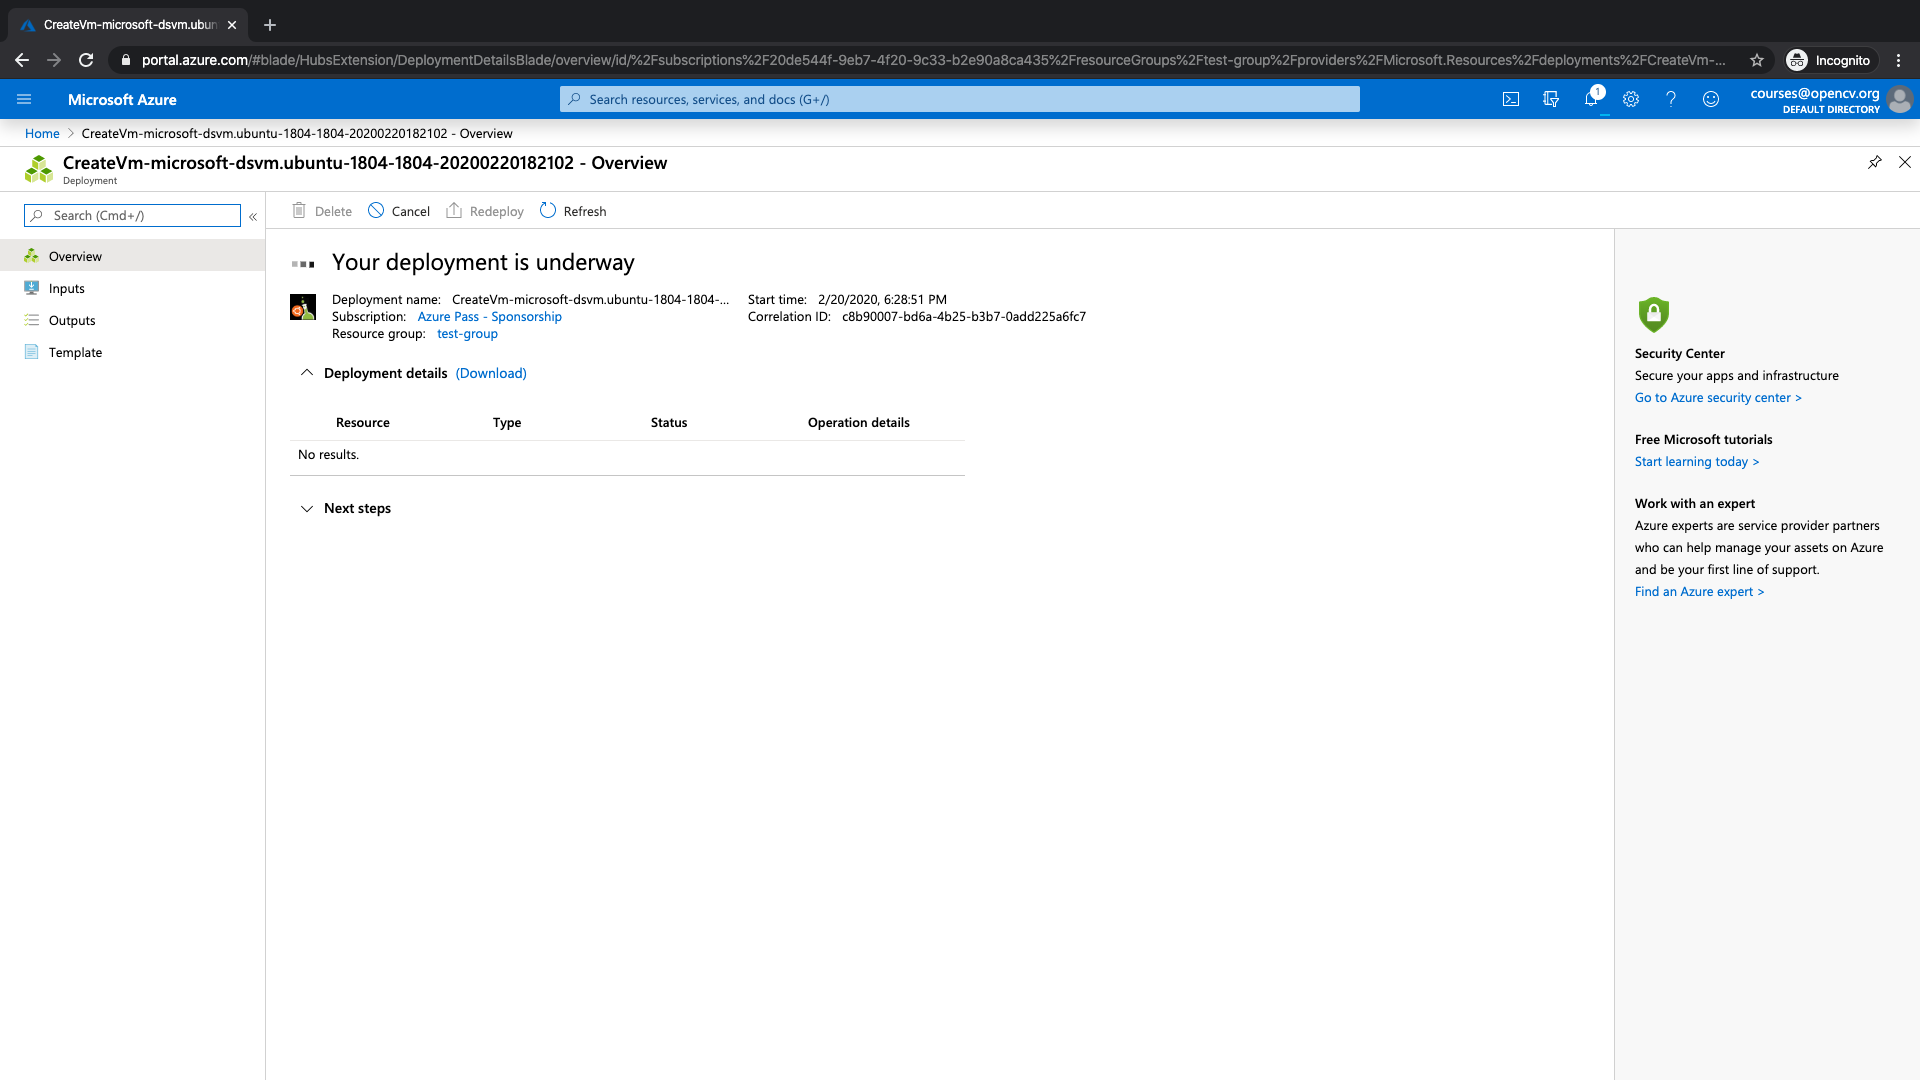
\includegraphics[scale=0.20]{figures/vm24}
%\caption{\small \sl . \cite{Mallick m.fl. 2020} \label{fig:azure}}
\end{center}
\end{figure}

20. Check your instance
Once the deployment is done,  you can check out your brand new instance. Click on Go to Resource. ( You can also click on the Home button on top left ).

\begin{figure}[H]
\begin{center} 
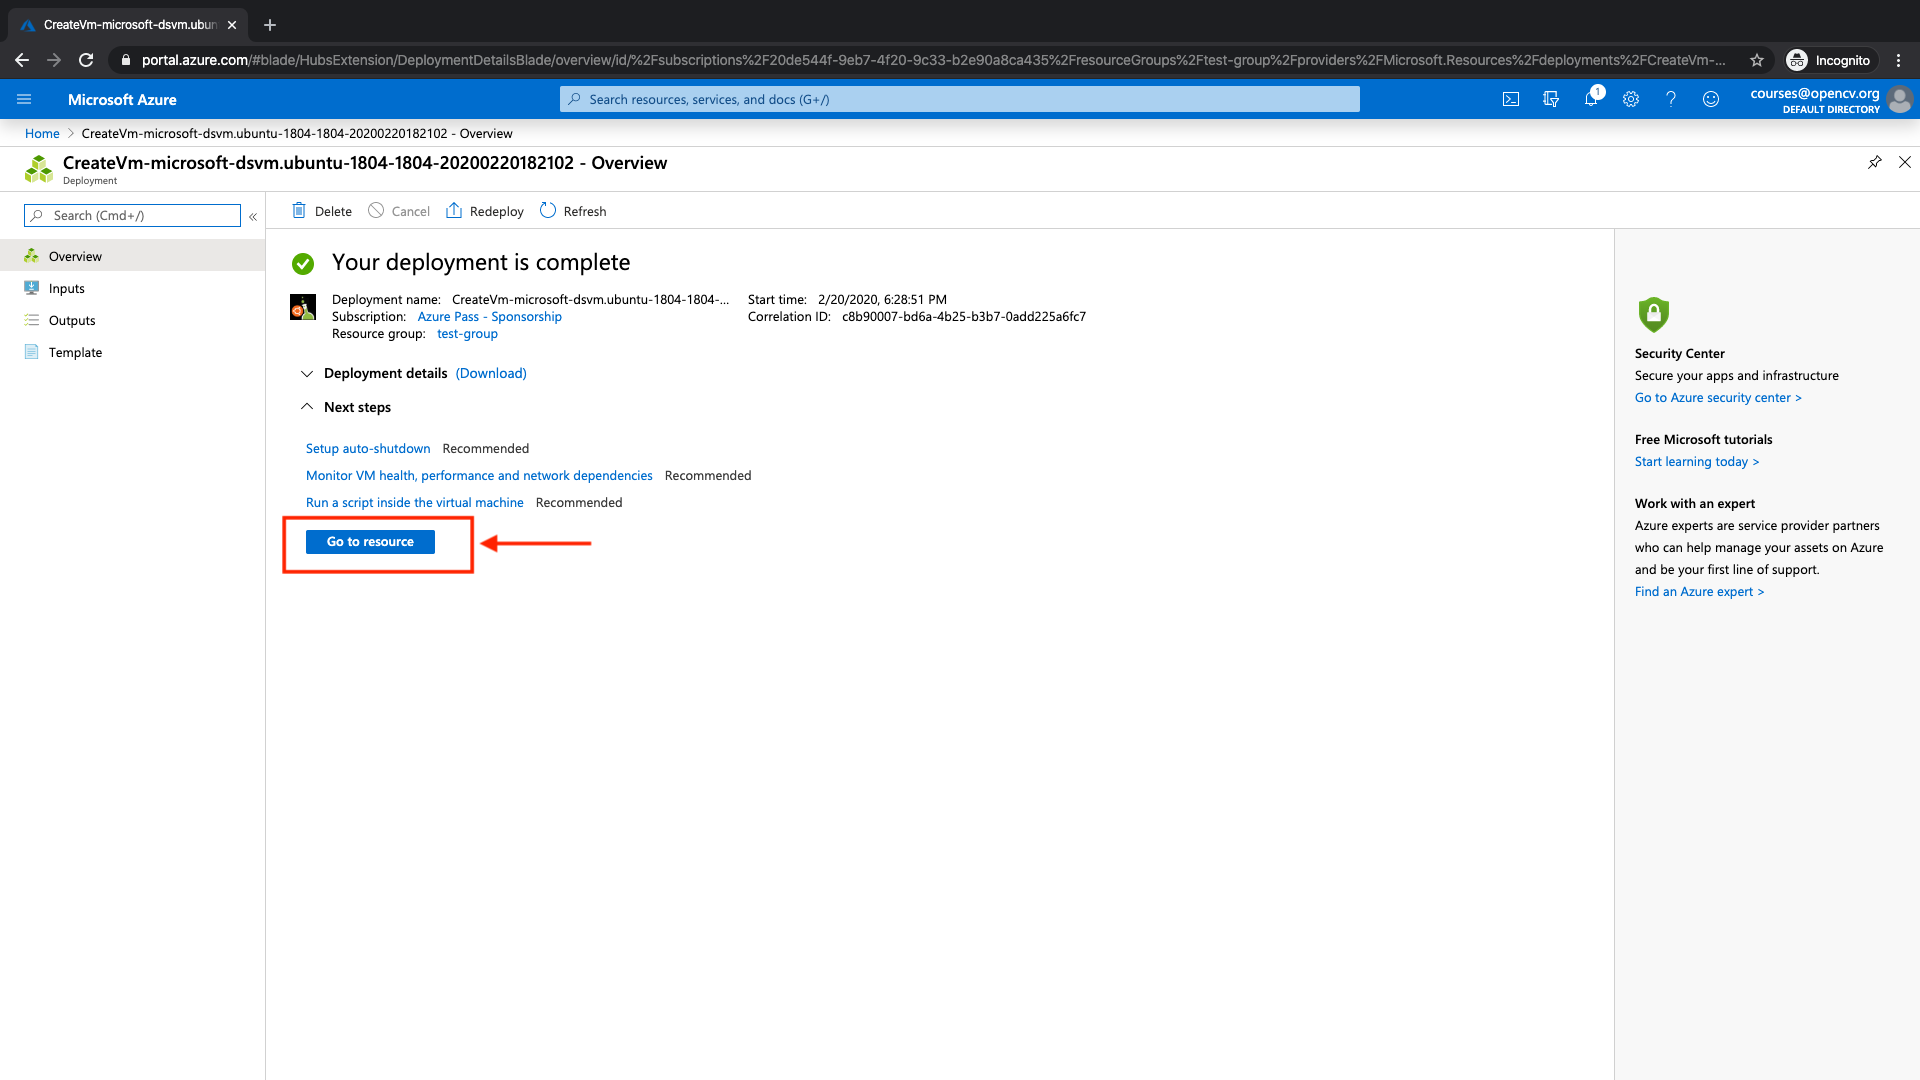
\includegraphics[scale=0.20]{figures/vm25}
%\caption{\small \sl . \cite{Mallick m.fl. 2020} \label{fig:azure}}
\end{center}
\end{figure}

\begin{figure}[H]
\begin{center} 
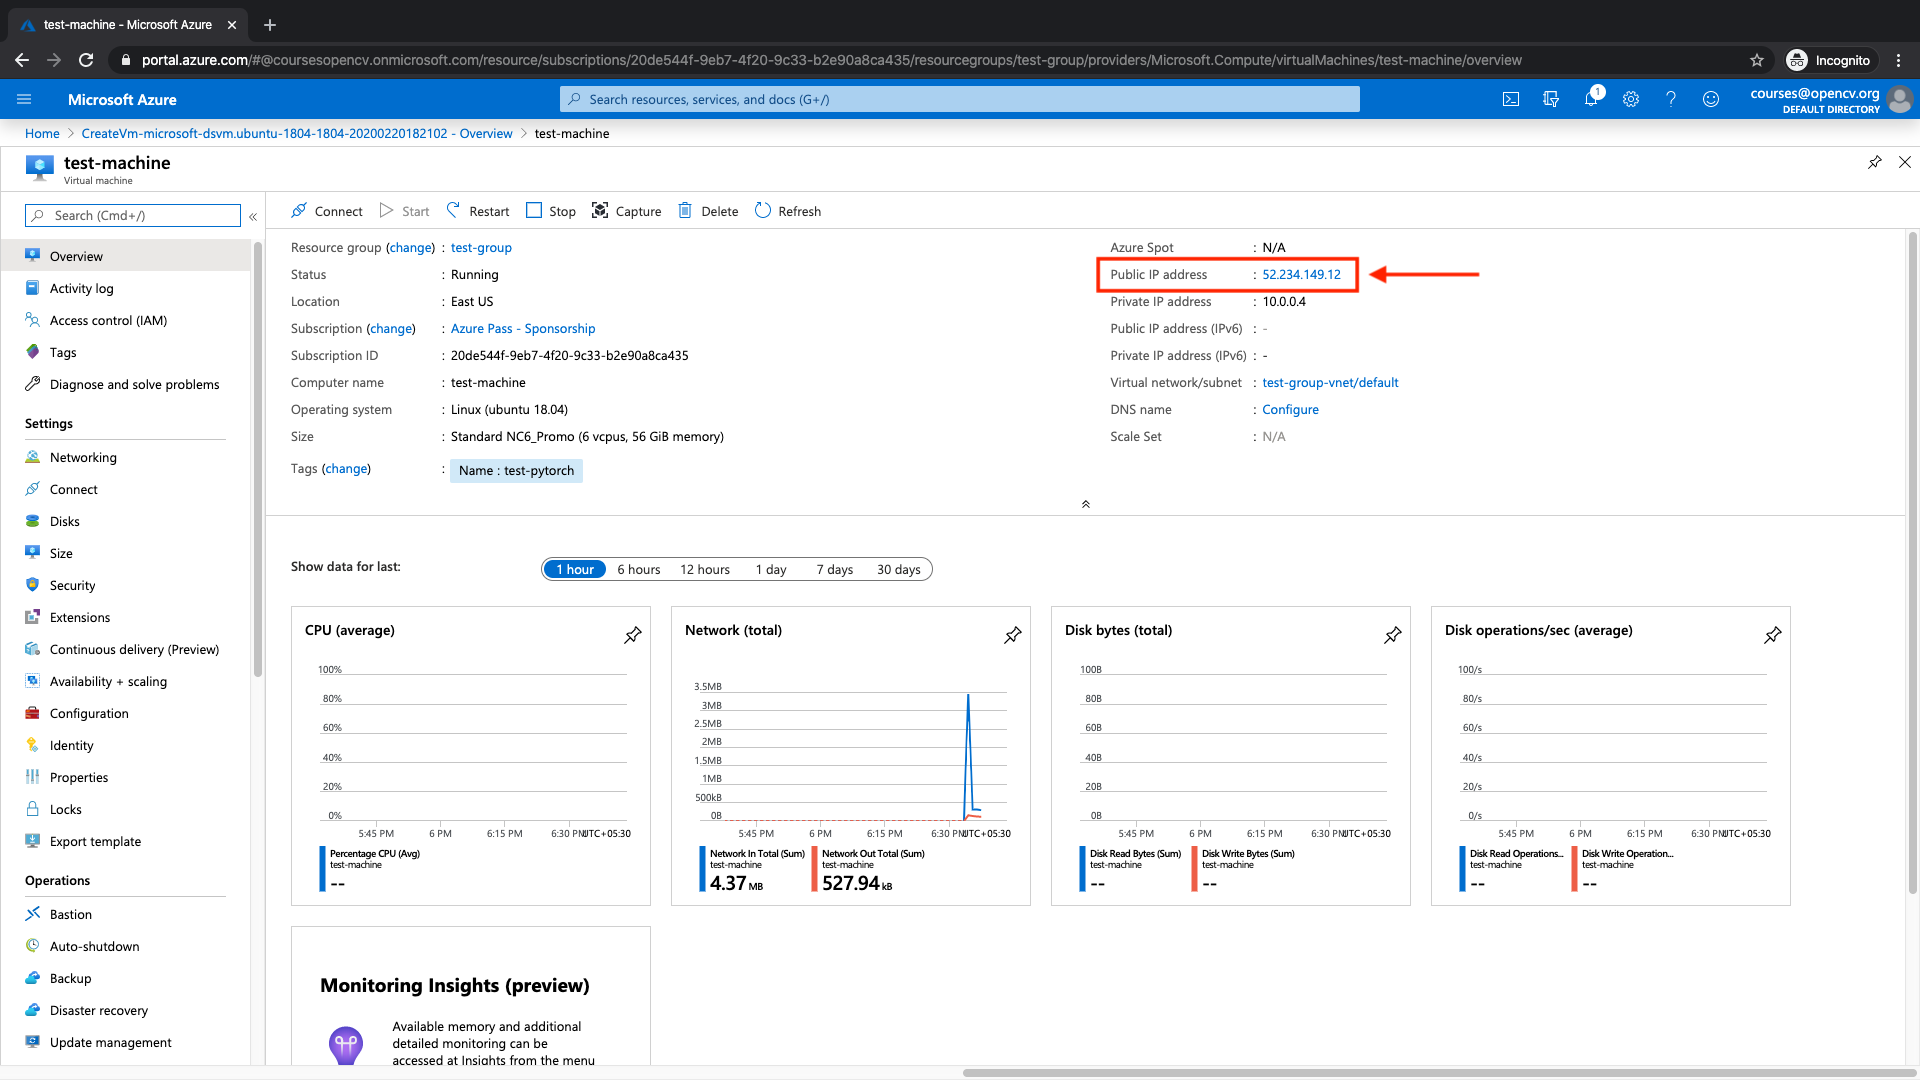
\includegraphics[scale=0.20]{figures/vm26}
%\caption{\small \sl . \cite{Mallick m.fl. 2020} \label{fig:azure}}
\end{center}
\end{figure}

You can see that your instance is created and it has been assigned a public IP address which you can use to login.
